\documentclass[11pt]{thesistemp}
\usepackage[italian]{babel}
\usepackage[utf8]{inputenc}
\usepackage{hyperref}
\usepackage[export]{adjustbox}
\usepackage{subcaption}
\usepackage{graphicx}
  \graphicspath{ {../media/} }
\usepackage{wrapfig}
\usepackage{color}
  \definecolor{dkgreen}{rgb}{0,0.6,0}
  \definecolor{gray}{rgb}{0.5,0.5,0.5}
  \definecolor{mauve}{rgb}{0.58,0,0.82}
\usepackage{listings}
\lstset{
  frame=tb,
  aboveskip=3mm,
  belowskip=3mm,
  showstringspaces=false,
  columns=flexible,
  numbers=none,
  numberstyle=\tiny\color{mauve},
  keywordstyle=\color{blue},
  commentstyle=\color{dkgreen},
  stringstyle=\color{mauve},
  breaklines=true,
  breakatwhitespace=true,
  tabsize=3
}

% Copyright 2017 Sergei Tikhomirov, MIT License
% https://github.com/s-tikhomirov/solidity-latex-highlighting/

\usepackage{listings, xcolor}

\definecolor{verylightgray}{rgb}{.97,.97,.97}

\lstdefinelanguage{Solidity}{
	keywords=[1]{anonymous, assembly, assert, balance, break, call, callcode, case, catch, class, constant, continue, constructor, contract, debugger, default, delegatecall, delete, do, else, emit, event, experimental, export, external, false, finally, for, function, gas, if, implements, import, in, indexed, instanceof, interface, internal, is, length, library, log0, log1, log2, log3, log4, memory, modifier, new, payable, pragma, private, protected, public, pure, push, require, return, returns, revert, selfdestruct, send, solidity, storage, struct, suicide, super, switch, then, this, throw, transfer, true, try, typeof, using, value, view, while, with, addmod, ecrecover, keccak256, mulmod, ripemd160, sha256, sha3}, % generic keywords including crypto operations
	keywordstyle=[1]\color{blue}\bfseries,
	keywords=[2]{address, bool, byte, bytes, bytes1, bytes2, bytes3, bytes4, bytes5, bytes6, bytes7, bytes8, bytes9, bytes10, bytes11, bytes12, bytes13, bytes14, bytes15, bytes16, bytes17, bytes18, bytes19, bytes20, bytes21, bytes22, bytes23, bytes24, bytes25, bytes26, bytes27, bytes28, bytes29, bytes30, bytes31, bytes32, enum, int, int8, int16, int24, int32, int40, int48, int56, int64, int72, int80, int88, int96, int104, int112, int120, int128, int136, int144, int152, int160, int168, int176, int184, int192, int200, int208, int216, int224, int232, int240, int248, int256, mapping, string, uint, uint8, uint16, uint24, uint32, uint40, uint48, uint56, uint64, uint72, uint80, uint88, uint96, uint104, uint112, uint120, uint128, uint136, uint144, uint152, uint160, uint168, uint176, uint184, uint192, uint200, uint208, uint216, uint224, uint232, uint240, uint248, uint256, var, void, ether, finney, szabo, wei, days, hours, minutes, seconds, weeks, years},	% types; money and time units
	keywordstyle=[2]\color{teal}\bfseries,
	keywords=[3]{block, blockhash, coinbase, difficulty, gaslimit, number, timestamp, msg, data, gas, sender, sig, value, now, tx, gasprice, origin},	% environment variables
	keywordstyle=[3]\color{violet}\bfseries,
	identifierstyle=\color{black},
	sensitive=false,
	comment=[l]{//},
	morecomment=[s]{/*}{*/},
	commentstyle=\color{gray}\ttfamily,
	stringstyle=\color{red}\ttfamily,
	morestring=[b]',
	morestring=[b]"
}

\lstset{
	language=Solidity,
	backgroundcolor=\color{verylightgray},
	extendedchars=true,
	basicstyle=\footnotesize\ttfamily,
	showstringspaces=false,
	showspaces=false,
	numbers=left,
	numberstyle=\footnotesize,
	numbersep=9pt,
	tabsize=2,
	breaklines=true,
	showtabs=false,
	captionpos=b
}


%----------------------------------------------------------------------------------------
%	TITLE
%----------------------------------------------------------------------------------------

\title{Servizi di supporto alle transazioni su Blockchain Ethereum}
\creationdate{10 Novembre 2018}
\redactedby{Aaron Cesaro}
\begin{document}
\maketitle
\pagebreak
%----------------------------------------------------------------------------------------
%	ABSTRACT
%----------------------------------------------------------------------------------------
\begin{abstract}
Questo documento si presenta come Tesi di Laurea triennale per il corso di laurea in informatica dello studente Aaron Cesaro. In esso \`e contenuta una relazione dettagliata dell’attivit\`a di stage svolta presso l’azienda Sgame SA, situata a Lugano (Svizzera). Durante il tirocinio, della durata complessiva di 300 ore, ogni abiettivo prefissato \`e stato raggiunto con successo, permettendo allo studente di acquisire dettagliate conoscenze sulle tecnologie e le metodologie di sviluppo utilizzate dalla società.
Particolare enfasi è stata data alla comprensione ed all'utilizzo della blockchain \textit{Ethereum} e di tutti i sevizi di supporto necessari alla corretta integrazione dello stesso all'interno della piattaforma \textit{Sgame Pro}.
\end{abstract}

\tableofcontents

%----------------------------------------------------------------------------------------
%	INTRODUZIONE
%----------------------------------------------------------------------------------------

\section{Introduzione}

\subsection{Contenuto del documento}

All'interno del docuemento verrano trattati i seguenti argomenti: 
\begin{itemize}
	\item \textbf{Capitolo 2: Blockchain network:} verrà descritta la rete \textit{blockchain}, le tecnologie che ne permettono il funzionamento, le logiche di base su cui si fondano le transazioni le principali differenze tra le piattaforme \textit{Bitcoin} ed \textit{Ethereum} ed una panoramica sul funzionamento di \textit{Ethereum} stessa.
	\item \textbf{Capitolo 3: La piattaforma Sgame Pro:} in questo capitolo verrà presentata l'applicazione \textit{Sgame Pro} e l'utilizzo di \textit{Ethereum} all'interno della stessa. Verrà inoltre data una visione d'insieme dell'applicazione, oltre a giustificare le motivazioni alla base dello sviluppo del servizio \textit{Token Value}.
	\item \textbf{Capitolo 4: Token Value service:} qui viene trattata progettazione e sviluppo del principale servizio realizzato durante il tirocinio, corredato dall'analisi dei requisiti imposti e dall'integrazione dello stesso nella piattaforma.
	\item \textbf{Capitolo 5: Ethereum Testnet:} verranno descritte dettagliatamente la creazione e l'integrazione delle \textit{testnet} di tipo \textit{private} e \textit{public}, oltre ad una panoramica sugli utilizzi e le necessità di utilizzo delle stesse.
	\item \textbf{Capitolo 6: Considerazioni finali:} in questa sezione verranno espresse alcune riflessioni sull'andamento del tirocinio e su obiettivi e traguardi raggiunti durante il suo svolgimento.
\end{itemize}

%----------------------------------------------------------------------------------------
%	BLOCKCHAIN
%----------------------------------------------------------------------------------------
\pagebreak
\section{Blockchain network}

\subsection{la tecnologia Blockchain}

\subsubsection{Definizione}

\textit{Blockchain} è una tecnologia che permette la creazione ed amministrazione di un grande database
distribuito tramite la gestione di transazioni condivisibili tra più nodi di una rete peer-to-peer.
Si tratta quindi di un database strutturato in blocchi (\textit{block}) che sono tra loro collegati (\textit{chain}) in modo che ogni transazione avviata sulla rete debba essere validata dalla rete stessa. 
In estrema sintesi la \textit{blockchain} è rappresentata da una catena di blocchi che
contengono e gestiscono più transazioni facendo uso della crittografia per rendere sicuro
l’immagazzinamento di dati ed il trasferimento di strumenti di valuta.\\\\
Pur essendo quest'ultima la definizione ``formale'' di \textit{blockchain}, ritengo che essa non evidenzi con chiarezza e semplicità cosa effettivamente una \textit{blockchain} sia.\\
Proverò quindi a scomporre ed analizzare la prima parte della definizione per rendere più fruibile il concetto.

\subsubsection{Server based e P2P}
La rete che normalmente viene utilizzata tutti i giorni per navigare in internet è quasi sempre \textit{server based} [\textbf{Figura~\ref{fig:server-based-net}}].\\
La peculiarità di questo sistema è che tutte le informazioni sono contenute in un solo posto, il \textit{Server} (da qui il nome \textit{server based}), il quale spesso gestisce un database che esercita il ruolo di archivio per l'immagazzinamento di dati ed effettua su di essi ricerche qualora vengano richiesti.
%----------------------------------------------------------------------------------------
%	FIGURA 1
%----------------------------------------------------------------------------------------
\begin{figure}[h]
    \centering
    \begin{subfigure}[h]{0.3\textwidth}
        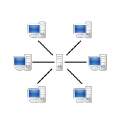
\includegraphics[width=\textwidth]{server-based-net.png}
        \caption{Server based network}
        \label{fig:server-based-net}
    \end{subfigure}\qquad
    \begin{subfigure}[h]{0.3\textwidth}
        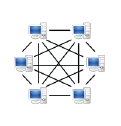
\includegraphics[width=\textwidth]{p2p-based-net.png}
        \caption{P2P based network}
        \label{fig:p2p-based-net}
    \end{subfigure}
    \caption{Tipologie di network}
    \label{fig:net}
\end{figure}\\\\
A differenza di una rete \textit{server based}, in una rete \textit{peer-to-peer} [\textbf{Figura~\ref{fig:p2p-based-net}}] (anche detta \textit{P2P}) non esiste la presenza di un server centrale che invia informazioni e tutti i dati vengono scambiati direttamente tra i nodi collegati alla rete. Ogni utente è quindi un \textit{client} ed un \textit{server} contemporaneamente.
Proprio per questa duplice funzione ogni dispositivo connesso viene detto \textit{nodo} della rete.\\
La sostanziale differenza tra le due tipologie di rete risiede nel fatto che mentre nel primo caso il \textit{server} contiene tutte le informazioni, nel secondo sono tutti e soli i \textit{client} a contenere i dati.\\
Ciò significa che nel primo caso il proprietario del \textit{server} può aggiungere, modificare o eliminare i dati che sono contenuti in esso, mentre nel secondo, anche se un nodo cancella o modifica i propri dati, gli altri nodi conterranno comunque tutte le informazioni originali. Da qui il termine distribuito.\\
\`E ora possible riprendere in mano la definizione originale: \textit{blockchain} è una tecnologia che permette di creare e gestire un grande archivio di informazioni, non contenute in un unico posto, ma del quale esiste una copia in ogni nodo connesso alla rete.

\subsection{Blockchain e Bitcoin}

\subsubsection{Ledger}
In letteratura è ritenuto più intuitivo usare \textit{Bitcoin} (\textit{BTC}) per esporre, tramite esempi semplificati, il funzionamento di una \textit{blockchain}.\\
Un \textit{Bitcoin} è una singola unità di valuta digitale che, proprio come l'\textit{Euro} non ha valore intrinseco, se non quello intenzionalmente attribuitogli grazie al consenso di scambio per l'acquisizione di beni o servizi.\\
%----------------------------------------------------------------------------------------
%	FIGURA 2
%----------------------------------------------------------------------------------------
\begin{wrapfigure}{r}{0.35\textwidth}
	\vspace{-31pt}
	\begin{center}
    	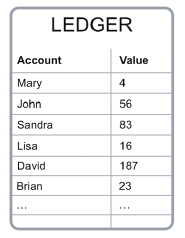
\includegraphics[width=0.37\textwidth]{ledger.png}
  	\end{center}
  	\vspace{-10pt}
  	\caption{Ledger}
  	\label{fig:ledger}
  	\vspace{-30pt}
\end{wrapfigure}
Per tenere traccia della quantità di \textit{Bitcoin} che ogni utente possiede si utilizza ciò che viene definito un \textit{Ledger} (libro mastro), che altro non è che un file in cui viene tenuta traccia di tutte le transazioni.
Il \textit{ledger} non è contenuto in un server centrale come ad esempio quello di una banca, ma ne esiste una copia in ogni nodo partecipante alla rete. In [\textbf{Figura~\ref{fig:ledger}}] è riportato, anche se in modo estremamente semplificato, un esempio di \textit{ledger}. 
Anche se nella realtà un ledger è molto diverso da quello in figura, nella pratica il disegno rappresenta fedelmente la funzione principale ricoperta da ogni copia del \textit{ledger} posseduta dai singoli nodi.
Nella colonna \textbf{Account} viene riportato il nome del proprietario dei \textit{Bitcoin}, mentre nella colonna \textbf{Value} è indicata la quantità posseduta da ognuno dei partecipanti.\\\\\\\\\\\\
Mettiamo caso che David voglia inviare cinque \textit{Bitcoin} a Sandra.
Per farlo è necessario che David mandi un messaggio sulla rete, il quale contiene la richiesta di transazione ed il numero di Bitcoin da lui posseduti.
Come informazione aggiuntiva viene inoltre trasmessa la quantità di \textit{Bitcoin} che possederà Sandra nel caso in cui la transazione avesse luogo. 
Il messaggio viene raggiunto dai nodi vicini a David i quali aggiornano i propri ledger con il risultato della possibile transazione (cioè David -5 \textit{BTC} e Sandra +5 \textit{BTC}) e rinviano il messaggio ai nodi a loro adiacenti. 
In questo modo il messaggio si espande per tutta la rete.
%----------------------------------------------------------------------------------------
%	FIGURA 3
%----------------------------------------------------------------------------------------
\begin{figure}[h]\hfill
    \centering
    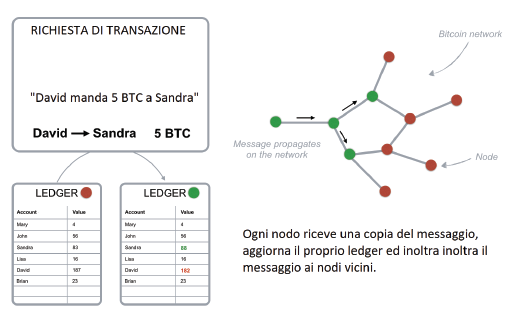
\includegraphics[width=\textwidth]{transaction.png}
    \caption{ Richiesta di transazione tra due nodi}
    \label{fig:transaction}
\end{figure}\\
Il fatto che il ledger sia mantenuto da tutti i nodi implica tre cose fondamentali, che stanno alla base del concetto della blockchain:
\begin{itemize}
\item  tutti sono a conoscenza di tutte le transazioni che avvengono sulla rete;
\item se la transazione non và a buon fine nessuno se ne prende la responsabilità in quanto non esiste un’entità centrale che si prenda carico dell’esito delle transazioni;
\item non esiste il bisogno di garanzie o fiducia in quanto la sicurezza è ottenuta tramite particolari funzioni matematiche estremamente sicure.
\end{itemize} 
\pagebreak

\subsubsection{Transazioni}
Perchè una transazione possa avere luogo è necessario ciò che viene definito un \textit{Wallet} (portafogli), ossia un software che permetta di depositare e scambiare scriptovaluta, tra cui \textit{Bitcoin}.
Poichè deve essere possibile solo ed esclusivamente al proprietario di un determinato \textit{Wallet} inviare i propri \textit{Bitcoin}, ogni \textit{Wallet} è protetto tramite una tecnica crittografica che usa una coppia di chiavi tra loro connesse.
Esse prendono il nome di chiave privata (\textit{private key}) e chiave pubblica (\textit{public key}).
%----------------------------------------------------------------------------------------
%	FIGURA 4
%----------------------------------------------------------------------------------------
\begin{figure}[h]\hfill
    \centering
    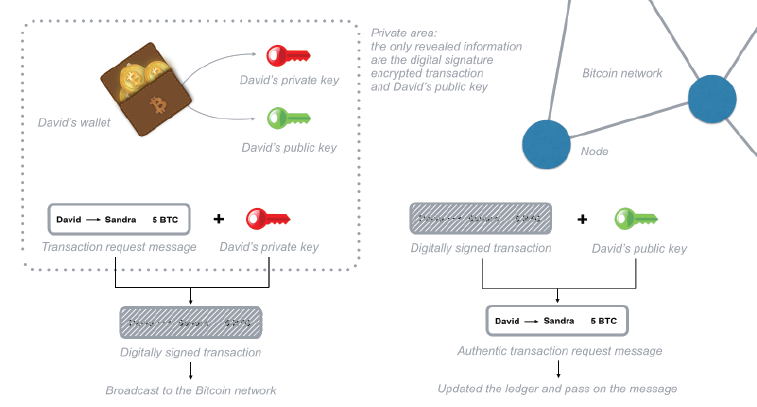
\includegraphics[width=\textwidth]{public-private-keys.png}
    \caption{Verifica della transazione tramite chiavi}
    \label{fig:pkey}
\end{figure}\\
Ogni messaggio in uscita da un singolo indirizzo viene criptato con una chiave privata il quale, una volta derivata la corrispondente chiave pubblica con cui è possibile identificare univocamente l'indirizzo di partenza (\textit{from}),deve poi essere validato dal nodo locale.
La validazione è necessaria per accertarsi che la transazione sia stata realmente messa sulla rete dal proprietario dell'account.
A questo punto solo i possessori della chiave pubblica associata potranno decifrare il messaggio.\\
Quando David vuole mandare 5 \textit{Bitcoin} a Sandra, deve inviare sulla rete il messaggio criptato con la sua chiave privata in modo che venga identificato come il possessore di un certo numero di \textit{Bitcoin} e sia di conseguenza l’unico a poter sbloccare il proprio \textit{Wallet}.
Tutti gli altri nodi validano la transazione, verificando tramite la chiave pubblica di David che la richiesta di inviare valuta sia effettivamente partita da lui.
In questo modo si ottiene la validazione della transazione.
In altre parole per poter inviare un \textit{Bitcoin} è necessario provare alla rete di essere i possessori dell'indirizzo da cui partono i \textit{Bitcoin}.\\
Nella rete inoltre non viene tenuto conto del bilancio dei singoli utenti, ma vengono semplecemente registrate le transazioni che avvengono.
La verifica di una transazione in questo modo si riduce semplicemente al controllo di tutte le transazioni passate, effettuate dall’utente che vuole inviare una certa somma di \textit{Bitcoin}.

\subsubsection{Blocchi}
Su una \textit{blockchain} le transazioni vengono ordinate tramite accorpamento con altre transazioni avvenute in un lasso di tempo definito.
In altre parole più transazioni vengono raggruppate insieme ed inserite dentro a quello che viene chiamato \textit{Block} (Blocco). 
Ogni \textit{block} contiene quindi un definito numero di transazioni ed un collegamento al nodo precedente. 
In questo modo si viene a creare una catena di blocchi molto simile ad una \textit{linked list}.
Da qui il nome \textit{blockchain} (catena di blocchi).
%----------------------------------------------------------------------------------------
%	FIGURA 5
%----------------------------------------------------------------------------------------
\begin{figure}[h]\hfill
    \centering
    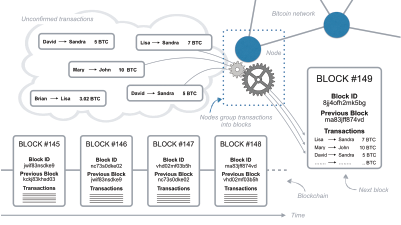
\includegraphics[width=\textwidth]{blocks.png}
    \caption{Rappresentazione di una blockchain}
    \label{fig:blocks}
\end{figure}\\
Le transazioni contenute nello stesso blocco sono considerate come avvenute nello stesso lasso temporale, mentre le transazioni che ancora non sono state raggruppate in un blocco sono considerate \textit{Unconfirmed}, cioè non ancora validate.\\ 
Ogni nodo della rete può raggruppare più transazioni e creare un blocco, suggerendo alla rete di inserirlo come prossimo blocco della catena. \\
Per essere effettivamente inserito nella rete un blocco deve contenere la soluzione ad un complesso problema matematico che, per essere risolto richiede una grossa potenza di calcolo, ed un pò di fortuna.
La risposta altro non è che un numero e l'unico modo per sapere quale sia il numero corretto da inserire consiste nel provarli tutti.
Il nodo che per primo risolve il problema acquisisce il diritto di inserire il prossimo blocco sulla catena e lo invia a tutti i nodi adiacenti.

\subsubsection{Mining}
A questo punto sorge spontaneo una domanda, ossia: "Se i Bitcoin posseduti da un account sono il risultato della somma di tutte le transazioni inviate e ricevute da quell'account, come è possibile ottenere altri \textit{Bitcoin}?"\\
La risposta a questa domanda é: "tramite il \textit{mining}".\\
Il \textit{mining} è l'attività svolta dai nodi definiti \textit{miners}, i quali, tramite la risoluzione di un complesso problema matematico, validano i blocchi, permettendo così a tutti i partecipanti alla rete di inviare e ricevere transazioni.\\
La validazione di un blocco nella pratica è una attività molto dispendiosa, sia in termini di energia elettrica che di consumo di banda.\\
Perchè la catena possa proseguire (cioè perchè possano essere effettuate nuove transazioni) è necessario che i blocchi siano inseriti nella catena e per farlo è necessario risolvere questo problema matematico.\\
Il modo escogitato per ripagare chi indovina il numero che valida il blocco (cioè svolge il lavoro di \textit{miner}) è una ricompensa in \textit{Bitcoin} da parte della rete. 
Questa ricompensa è ciò che incentiva le persone a provvedere al necessario lavoro computazionale per far continuare la catena e mantenere la rete utilizzabile. Senza i \textit{miners} i blocchi non potrebbero essere validati, la catena si fermerebbe e le transazioni non potrebbero più avere luogo.

\pagebreak
\subsection{Ethereum}

\subsubsection{Ethereum e Bitcoin}

Come \textit{Bitcoin}, \textit{Ethereum} è una \textit{public blockchain}.\\
Sebbene ci siano alcune significative differenze tecniche tra le due, la distinzione più importante da notare è che \textit{Bitcoin} ed \textit{Ethereum} differiscono sostanzialmente per scopo e capacità.\\
Il \textit{Bitcoin} è stato lanciato come valuta alternativa, o moneta digitale, ed offre una particolare applicazione della tecnologia \textit{blockchain}, ossia un sistema di pagamento elettronico.\\
\textit{Ethereum} invece viene principalmnte utilizzato per applicazioni decentralizzate tramite l'utilizzo degli \textit{Smart Contract}.\\
A differenza di \textit{Bitcoin}, \textit{Ethereum} utilizza due concetti di \textit{token}: il primo prende il nome di \textit{Ether} e corrisponde alla "moneta" effettivamente scambiata tra gli utenti della rete, il secondo viene invece utilizzato per pagare i \textit{miners}, i quali includono le transazioni nei blocchi, e prende il nome di \textit{gas}.

\subsubsection{Smart Contract}

Uno \textit{Smart Contract} è un programma che contiene un insieme di regole a cui le parti interessate accettano di aderire.\\
Nel caso in cui le regole definite all'interno di uno smart contract siano soddisfatte l'accordo tra le parti viene automaticamente applicato.\\
Il codice di uno \textit{Smart Contract} facilita, verifica e impone la negoziazione o l'esecuzione di un accordo o di una transazione e corrisponde alla forma più semplice di automazione decentralizzata.\\
Il successo di \textit{Ethereum} (e la più grande differenza con \textit{Bitcoin}) dipende proprio dal concetto di \textit{Smart Contract}. grazie a cui è possible programmare una serie definita di azioni che vengono attuate se e solo se le condizioni in esso contenute vengono soddisfatte.\\\\
Gli \textit{Smart Contract} sono spesso scritti in un linguaggio di programmazione chiamato \textit{Solidity}, estremamente simile a \textit{JavaScript} e \textit{C++}.\\
Il codice degli \textit{Smart Contract} viene poi eseguito in \textit{Ethereum} tramite una particolare macchina virtuale che prende il nome di \textit{EVM} (\textit{\textbf{E}thereum \textbf{V}irtual \textbf{M}achine})
\pagebreak

\subsection{Ethereum Virtual Machine}

Una macchina virtuale (\textit{virtual machine}) ha essenzialmente lo scopo di creare un livello di astrazione tra il codice in esecuzione e la macchina fisica che lo esegue.\\
Questo livello è necessario per migliorare la portabilità del software, oltre a garantire la separazione tra applicazioni ed host.\\
La \textit{EVM} è stata progettata come \textit{runtime environment} per l'esecuzione degli \textit{Smart Contract} basati su \textit{Ethereum} e può essere pensata come una \textit{Semi-Touring complete machine}.\\
Viene definita \textit{"Semi-Touring complete"} in quanto i calcoli eseguiti sono delimitati dal \textit{gas}, ossia dal costo addizionale associato ad ogni transazione.\\
Il pagamento di una certa somma di \textit{gas} funge da costo associato all'esecuzione e, se il costo supera la somma pagata, la transazione non ha luogo.\\
Questo si traduce in una forma estremamente efficace per la prevenzione di attacchi di tipo \textit{Ddos} (\textit{Denial-of-service}) o errori logici come i cicli infiniti.\\
Il codice degli \textit{Smart Contract} non possono essere eseguiti direttamente dalla \textit{EVM}.
Innanzitutti è prima necessario che siano compilati in un linguaggio di basso livello (codice macchina) che prende il nome di \textit{opcode}.

\subsubsection{Opcode}

L'\textit{EVM} utilizza una serie di istruzioni macchina necessarie all'esecuzione di attività specifiche.\\
Ogni istruzione (\textit{opcode}) viene rapresentata con (1) byte, ossia due caratteri esadecimali.\\
Ciò comporta che possono esistere un totale massimo di 256 diversi codici operativi.\\
All'interno della \textit{EVM} esistono istruzioni come \textit{PUSH}, 
Al fine di salvare efficientemente gli \textit{opcode} essi vengono codificati in quello che viene chiamato \textit{bytecode} e, ad ogni codice operativo viene assegnato un byte (ad esempio, STOP è 0x00).\\
%----------------------------------------------------------------------------------------
%	FIGURA 5
%----------------------------------------------------------------------------------------
\begin{figure}[h]
    \centering
    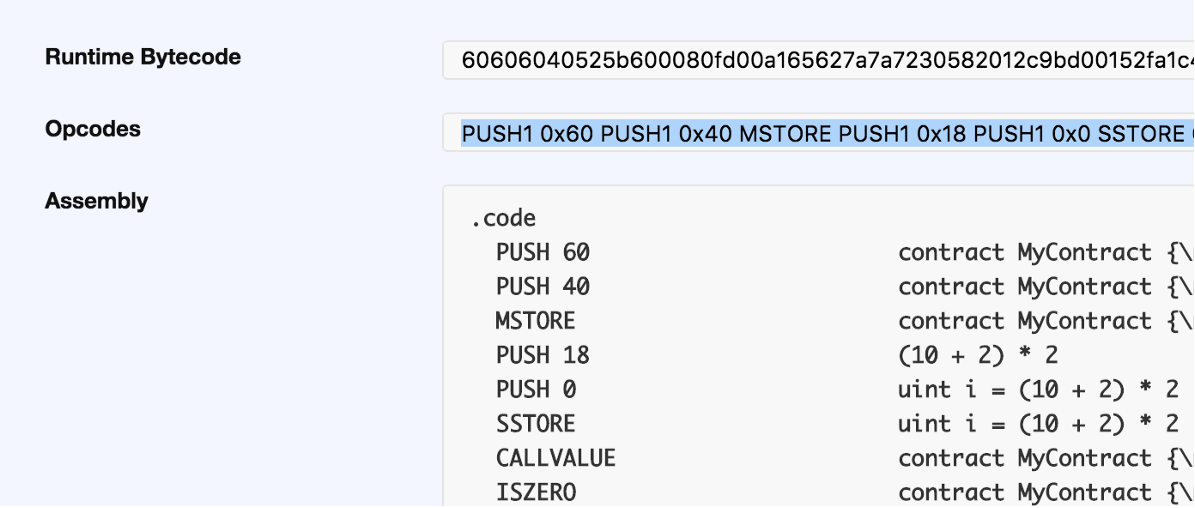
\includegraphics[scale=.5]{bytecode-opcode.png}
    \label{fig:bytecode-opcode}
\end{figure}
\linebreak

\subsubsection{Bytecode}

Il \textit{bytecode} della \textit{EVM} rappresenta il codice compilato degli \textit{Smart Contract} ed è necessario per dare la priorità di esecuzione delle istruzioni.\\
%----------------------------------------------------------------------------------------
%	FIGURA 5
%----------------------------------------------------------------------------------------
\begin{figure}[h]\hfill
    \centering
    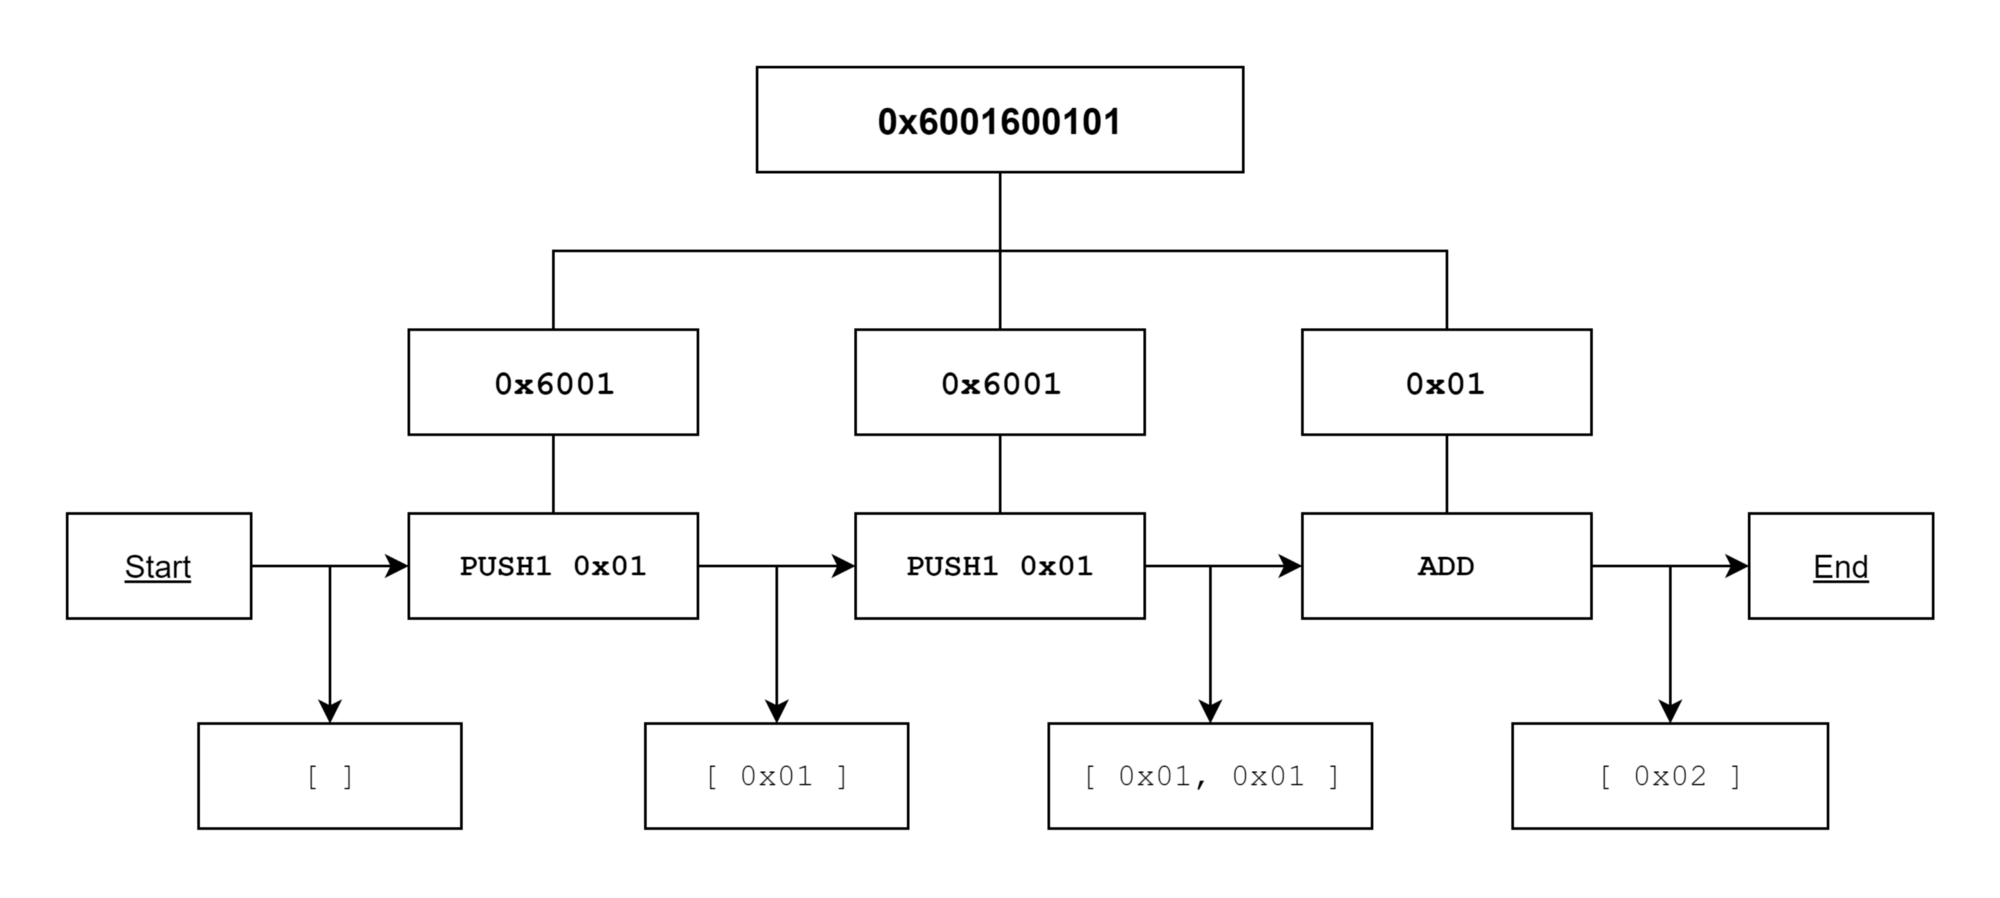
\includegraphics[width=\textwidth]{bytecode.png}
    \label{fig:bytecode}
\end{figure}
\linebreak
Questa logica permette alla \textit{EVM} di attuare come una macchina a stati.\\
Durante l'esecuzione infatti il \textit{bytecode} è diviso in bytes, i quali sono enterpretati ad uno ad uno.\\

\subsubsection{Application Binary Interface}

Le chiamate verso \textit{Smart Contract} richiedono un \textbf{ABI} (\textit{\textbf{A}pplication \textbf{B}inary \textbf{I}nterface}), ossia un insieme di dati che documenti tutte le funzioni e gli eventi disponibili nello \textit{Smart Contract} stesso, inclusi gli input e gli output necessari alle chiamate.\\
L'\textit{ABI} utilizza un formato \textit{JSON} il quale viene rilasciato come \textit{output} della compilazione del codice sorgente \textit{Solidity}.
%----------------------------------------------------------------------------------------
%	Sgame Pro
%----------------------------------------------------------------------------------------

\section{La piattaforma Sgame Pro}
%----------------------------------------------------------------------------------------
%	FIGURA 5
%----------------------------------------------------------------------------------------
\begin{figure}[h]\hfill
    \centering
    
\includegraphics[width=\textwidth]{sgamepro-logo.png}
    \label{fig:sgamepro}
\end{figure}

\subsection{Overview}

\textit{Sgame Pro} è un aggregatore di \textit{mobile games} di proprietà di \textit{Sgame SA}, con sede a Lugano, Svizzera.\\
In sviluppo dal 2016, Sgame Pro ha lanciato con successo la sua \textit{Alpha version} nel 2017, raggiungendo oltre 50.000 download senza alcuna spesa di marketing.\\
\textit{Sgame Pro} è interamente focalizzato sull'industria dei \textit{mobile games} e ha sviluppato due importanti innovazioni tecniche:
\begin{itemize}
	\item Consentire ai giocatori di essere remunerati con un nuovo utility token (\textit{SGM}) semplicemente giocando con il proprio cellulare ai titoli proposti;
	\item Aggregare il frammentato settore dei \textit{publisher}, indipendenti e non, in un'unica piattaforma di gioco \textit{one-stop-shop}.
\end{itemize}
 L'\textit{SGM} (token di tipo \textit{utility} basato sullo standard \textit{Ethereum ERC-20}) sarà l'unico modo per accedere ai servizi e beneficiare di tutte le funzinalità messe a disposizione degli utenti, oltre ad essere il metodo di pagamento unico per tutte le transazioni all'interno dell'ecosistema della piattaforma.\\
All'interno dell'applicazione i giocatori non solo avranno l'opportunità di trovare tutti gli ultimi titoli mobile resi disponibli, ma avranno anche l'opportunità di sfidare gli altri utenti sia in privato che tramite la funzionalità di \textit{Public Challenge}.\\
Quest'ultima innovazione è davvero dirompente dato che il 78\% del mercato dei giochi mobile è single player, mentre la maggior parte delle entrate derivano da giochi multiplayer.\\
Gli \textit{Influencers} di \textit{Sgame Pro} includono \textit{Pewdiepie}, \textit{Tweakbox} e molti altri, con oltre 80 milioni di seguaci altamente coinvolti e sparsi in tutto il mondo.\\ 

\subsection{Funzionalità principali}

\subsubsection{Challenges}

Le \textit{Challenges} sono una delle caratteristiche principali di \textit{Sgame Pro}.\\
Esse consentono infatti di sfidare gli altri giocatori all'interno della piattaforma e di guadagnare gli \textit{SGM} messi in palio per la sfida.\\
Le \textit{challenges} permettono inoltre di trasformare qualunque gioco da semplice \textit{single play} a \textit{multiplayer}, dando agli utenti la possibilità di sfidarsi in modalità asincrona.\\

%----------------------------------------------------------------------------------------
%	FIGURA 6
%----------------------------------------------------------------------------------------
\begin{figure}[h]\hfill
    \centering
    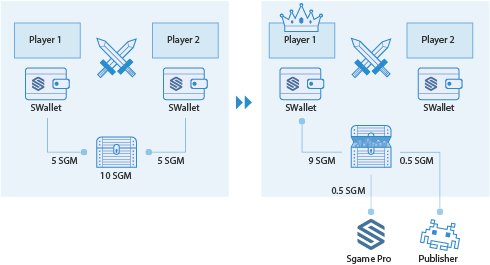
\includegraphics[width=\textwidth]{challenges.png}
        \caption{Funzionlità Challenges}
    \label{fig:challenges}
\end{figure}
All'interno dell'applicazione esistono due diverse tipologie di sfide:
\begin{itemize}
	\item \textbf{Private Challenges}: le quali consentono agli utenti di sfidarsi tra loro, scegliendo tutti i partecipanti alla competizione direttamente tra i propri \textit{Friends}, e mettendo in palio l'importo in \textit{SGM} desiderato;
	\item \textbf{Public Challenges}: le quali invece danno la possibilità di creare una sfida \textit{ad-hoc} a cui chiuque può partecipare, specificando il numero minimo/massimo di utenti necessario affinchè la sfida possa avere luogo.
\end{itemize}
\pagebreak

\subsubsection{Leaderboard}

La \textit{Leaderboard} è la classifica globale di punteggi ottenuti dagli utenti in uno specifico titolo.\\
Questa funzionalità consente ai giocatori di confrontare le proprie prestazioni con quelle degli avversari.\\
L'innovativo approccio di Sgame Pro a questa "classica" funzionalità consiste nell'esporre:
\begin{itemize}
	\item \textbf{Classifiche comuni tra iOS ed Android}: i giocatori possono finalmente competere tra loro indipendentemente dal sistema operativo utilizzato;
	\item \textbf{Classifiche premiate}: i giocatori che battono particolari record od obiettivi vengono premiati in \textit{SGM}.
\end{itemize}

\subsubsection{User Profile}
%----------------------------------------------------------------------------------------
%	FIGURA 7
%----------------------------------------------------------------------------------------
\begin{wrapfigure}{r}{0.2\textwidth}
	\vspace{-31pt}
	\begin{center}
    	
\includegraphics[width=0.2\textwidth]{user-profile.png}
  	\end{center}
  	\vspace{-10pt}
  	\caption{Profilo}
  	\label{fig:user-profile}
  	\vspace{-60pt}
\end{wrapfigure}
Ogni giocatore o \textit{influencer} avrà il proprio profilo utente dedicato contenente una panoramica di punteggi, tempi di gioco ed altre statistiche utili.\\
Il profilo utente contiene inoltre le seguenti informazioni:
\begin{itemize}
	\item livello dell'utente;
	\item numero di amici e \textit{followers};
	\item statistiche delle \textit{challenges};
	\item titoli giocati di recente;
	\item dati sugli avversari;
	\item dattagli sui guadagni.
\end{itemize}
\pagebreak

\subsubsection{Marketplace}

La sezione \textit{Marketplace} permette agli utenti della piattaforma \textit{Sgame Pro} di acquistare \textit{digital goods} (coupons, free subscriptions etc..) direttamente all'interno dell'applicazione.\\
\`E inoltre possibile fissare dei "\textit{target}", ossia scegliere un particolare oggetto all'interno del \textit{marketplace} e porsi come obiettivo il raggiungimento della cifra necessaria al suo acquisto.

\subsubsection{Wallet}

All'interno della funzionalità \textit{Wallet} l'utente può sempre tenere sotto controllo il suo patrimonio ed avere una panoramica dettagliata del flusso di cassa (in \textit{SGM}) del suo account.\\
\\
Da questa sezione è inoltre possibile trasformare gli \textit{SGM} guadagnati all'interno della piattaforma in criptovaluta fruibile all'interno della rete \textit{Ethereum}.\\
\`E infatti tramite questa funzinalità che entrano in gioco la \textit{blockchain} e tutti i servizi di supporto ad essa associati.
\pagebreak

\subsection{Sgame Pro ed Ethereum}

L'idea iniziale alla base dell'integrazione di \textit{Ethereum} all'interno della piattaforma \textit{Sgame Pro} prevedeva un'applicazione completamente decentralizzata (\textit{full decentralized}) a cui ogni movimento di \textit{SGM} corrispondeva una transazione su \textit{Ethereum}.\\\\
Questo approccio avrebbe portato numerosi benefici a livello di \textit{trust}, ma sarebbe stato altamente insostenibile per il \textit{business model} della società.\\
Infatti, come già detto, ogni transazione su \textit{Ethereum} richiede una determinata quantità di \textit{gas}, necessaria per l'esecuzione dello \textit{smart contract}, che deve essere aggiunta all'ammontare che si desidera trasferire.
In altre parole il costo di ogni transazione sarebbe stato maggiore dell'ammontare scambiato durante la transazione stessa.\\
Si è deciso quindi di utilizzare un sistema di remunerazione interno "classico", ossia tramite assegnazione a livello di database, dando però la possibilità agli utenti di transferire i propri guadagni sul proprio \textit{wallet} personale qualora lo desiderassero.

\subsubsection{Sgame Token}

\textit{Ethereum} è stato creato per essere un vero e proprio ambiente di sviluppo, infatti esso può essere utilizzato, tramite la creazione di appositi \textit{Smart Contract}, per creare criptovalute che si appoggino sulla sua \textit{currency} base, ossia l'\textit{Ether}.\\
Le criptovalute derivate da \textit{Ether}, dette anche \textit{token}, sono principalmente state utilizzate per l'attuazione delle \textit{ICO} (\textit{Initial Coin Offer}), ossia \textit{crowdfundig} attuati tramite la vendita di particolari criptovalute, utilizzate come finanziamenti al posto della moneta tradizionale (\textit{FIAT}).\\
Come già citato l'\textit{SGM} è il token utilizzato dalla piattaforma \textit{Sgame Pro}.\\
Esso è stato creato allo scopo di uniformare quelli che vengono definiti \textit{In-App purchase}, permettendo così agli utenti di poter acquistare qualunque tipo di beneficio, all'interno dei titoli presenti nella piattaforma, con una unica valuta.\\\\
L'\textit{SGM} si appoggia su quello che formalmente \textit{Ethereum} definisce lo \textit{Standard ERC-20}, ossia un'interfaccia che gli \textit{Smart Contract} possono implementare nel caso in cui si intenda utilizzare alcune tipologie di servizi offerti da \textit{Ethereum.}
%----------------------------------------------------------------------------------------
%	ERC-20 STANDARD
%----------------------------------------------------------------------------------------
\begin{lstlisting}[language=Solidity]
contract ERC20Interface {
   function totalSupply() public view returns (uint);
   function balanceOf(address tokenOwner) public view returns (uint balance);
   function allowance(address tokenOwner, address spender) public view returns (uint remaining);
   function transfer(address to, uint tokens) public returns (bool success);
   function approve(address spender, uint tokens) public returns (bool success);
   function transferFrom(address from, address to, uint tokens) public returns (bool success);

   event Transfer(address indexed from, address indexed to, uint tokens);
   event Approval(address indexed tokenOwner, address indexed spender, uint tokens);
}
\end{lstlisting}
L'interfaccia \textit{ERC-20} funge da contratto per il set minimo di funzionalità che si intende mettere a disposizione dopo la creazione (\textit{issuing}) ti un token derivato da \textit{Ethereum}.\\
La scelta di aderire a questo standard è stata guidata dall'altissima compatibilità con i vari \textit{Exchange} presenti oggigiorno sul mercato.

\section{Token Value Service}

\subsection{Overview}

\textit{Token Value} è un servizio di acquisizione e memorizzazione dello storico di valori di criptovalute sulle diverse piattaforme di scambio (\textit{Exchange}).\\
Il servizio espone delle \textit{API} pubbliche, utilizzate direttamente dalla piattaforma \textit{Sgame Pro}, per il calcolo delle vincite dei giocatori ed il prezzo dei beni acquistabili nella sezione \textit{Marketplace}. \\
Grazie all'implementazione di questo servizio il sistema può applicare le logiche di business basate sul calcolo del prezzo presentato all'interno dell'applicazione, in modo da assicurare equità nell'attribuzione di \textit{SGM} e coerenza del valore riportato sugli oggetti acquistabili all'interno della stessa.\\
Le funzionalità principali del servizio comprendono:
\begin{itemize}
	\item ottenimento del valore del token \textit{SGM} tramite l'utilizzo delle API messe a disposizione di ciascun exchange;
	\item memorizzazione persistente dei valori ottenuti su database PostgreSQL;
	\item caching dei valori per la diminuzione dei tempi di risposta;
	\item utilizzo e trasmissione di valori ottimali secondo le logiche di selezione approvate dalla società.
\end{itemize}
Il servizio rappresenta attualmente un tassello fondamentale per la società \textit{Sgame SA} in quanto il valore del token riportato e propagato all'intera applicazione ha un impatto estremamente concreto sui guadagni dell'intera società.\\\\
Una logica scorretta all'interno del servizio porterebbe irreparabilemente ad una erronea attribuizione delle vincite agli utenti e ad una possible perdita di denaro per la società.\\\\
Proprio per queste ragioni il servizio utilizza logiche estremamente semplici e facilmente testabili.
\pagebreak

\subsection{Pianificazione}

\begin{itemize}
	\item \textbf{Prima Settimana}(42,5 ore) – Incontro con il team di sviluppo, formazione sul funzionamento di Ethereum ed introduzione ai linguaggi C\# e Solidity;
	\item \textbf{Seconda Settimana}(42,5 ore) – Acquisizione delle informazioni necessarie alla realizzazione del servizio TokenValue ed ai servizi interni che utilizzerà ;
	\item \textbf{Terza Settimana}(42,5 ore) – Sviluppo della logica di acquisizione e memorizzazione persistente dei valori necessari all’utilizzo del servizio TokenValue.
	\item \textbf{Quarta Settimana}(42,5 ore) – Debugging e sviluppo della documentazione del servizio TokenValue. Entro il termine della settimana il tirocinante dovrà aver terminato e documentato il servizio sviluppato.
	\item \textbf{Quinta Settimana}(42,5 ore) – Creazione dell’interfaccia grafica necessaria agli analisti di Sgame per la visualizzazione dei valori di mercato della criptovaluta target.
\end{itemize}
\pagebreak

\subsection{Analisi dei requisiti}

\subsubsection{Notazioni}

Viene di seguito riportata la notazione che verrà utilizzata per l’identificazione dei requisiti classificati per utilità strategica: 
\begin{itemize}
	\item \textbf{Ob} – requisiti obbligatori, irrinunciabili per qualsiasi Stakeholders.
	\item \textbf{De} – requisiti desiderabili, aggiungono valore al prodotto.
\end{itemize}
Viene di seguito riportata la notazione che verrà utilizzata per l’identificazione dei requisiti classificati per verificabilità: 
\begin{itemize}
	\item \textbf{Vi} – requisiti vincolo, imposti dal cliente o dal sistema in cui lavora il software.
\end{itemize}

\subsubsection{Specifica dei requisiti}

\textbf{Obbligatori}:
\begin{itemize}
	\item \textbf{Ob001} – il prodotto \textit{Token Value} deve raccogliere i dati sui valori delle criptovalute tramite chiamata \textit{REST API} al servizio cryptocompare.
	\item \textbf{Ob002} – il prodotto \textit{Token Value} deve salvare dati persistenti sia sul valore attuale del token che sullo storico dei valori richiesti.
	\item \textbf{Ob003} – il prodotto \textit{Token Value} deve essere corredato da documentazione.
\end{itemize}
\textbf{Desiderabili}:
\begin{itemize}
	\item \textbf{De001} – il prodotto \textit{Token Value} deve essere documentato tramite\textit{ XML notation}.
	\item \textbf{De002} – il prodotto \textit{Token Value} deve essere facilmente configurabile sia in ambiente \textit{Development} che in ambiente \textit{Staging} tramite l’utilizzo di specifiche variabili d’ambiente.
\end{itemize}
\textbf{Vincolo}:
\begin{itemize}
	\item \textbf{Vi001} – il prodotto \textit{Token Value} deve essere realizzato nel linguaggio \textit{C\#} ed utilizzare \textit{PostgreSQL} per il salvataggio persistente dei dati.
\end{itemize}
\pagebreak

\subsection{Architettura}

L'architettura del servizio riprende fedelmente il modello utilizzato dagli altri servizi relativi ad \textit{Ethereum} sviluppati sulla piattaforma.\\\\
Ogni servizio è composto da due moduli separati:
\begin{itemize}
	\item \textbf{Public API}: interfaccia pubblica che espone \textit{API} di tipo \textit{REST} all'interno dell'ambiente stesso;
	\item \textbf{Core}: \textit{business logic} del servizio. Si occupa delle richieste verso i servizi esterni e dell'interfacciamento con il database. Nel modulo sono quindi compresi sia il \textit{Business Layer} che il \textit{Data Layer}.
\end{itemize}
%----------------------------------------------------------------------------------------
%	FIGURA 8
%----------------------------------------------------------------------------------------
\begin{figure}[h]\hfill
    \centering
    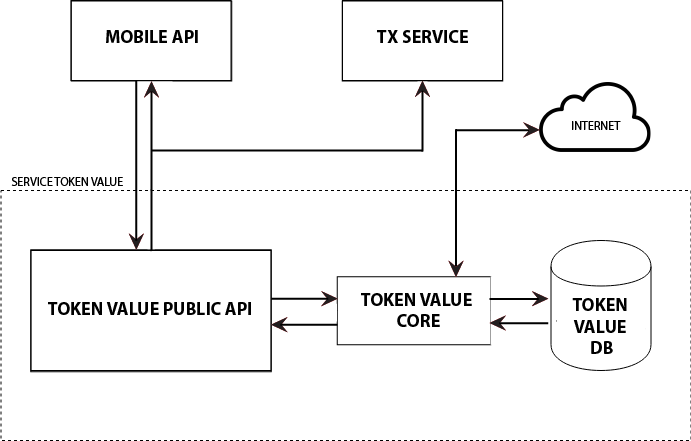
\includegraphics[width=\textwidth]{tkvalue-arch.png}
        \caption{Architettura del servizio Token Value}
    \label{fig:tkvalue-arch}
\end{figure}
Grazie a questa struttura a \textit{layers} si garantisce l'impossibilità di comunicazione diretta con la logica del servizio ed una netta separazione delle responsabilità all'interno del servizio stesso.\\
Il servizio \textit{Token Value} si interfaccia poi con il resto del backend dell'applicazione (quello che la compagnia ha deciso di chiamare \textit{Mobile API}), e con \textit{TX}, ossia il servizio che si occupa della comunicazione diretta con lo \textit{Smart Contract} interfacciandosi alla \textit{blockchain Ethereum}.

\subsection{Progettazione}
Viene di seguito esposto il diagramma delle classi (\textit{UML 2.0}) del servizio \textit{Token value}.\\
All'interno nel servizio è possibile mappare i due moduli riportati nello schema dell'architettura nel seguente modo:
\begin{itemize}
	\item \textbf{Public API} contiene la classe \textit{ValueController}, la quale funge da interfaccia interna e viene richiamata da \textit{Mobile API};
	\item \textbf{Core} comprende tutto il resto del servizio, ossia i \textit{Managers} ed i \textit{Repository}, necessari all'orchestrazione ed alla comunicazione con il database rispettivamente.
\end{itemize}
%----------------------------------------------------------------------------------------
%	FIGURA 9
%----------------------------------------------------------------------------------------
\begin{figure}[h]\hfill
    \centering
    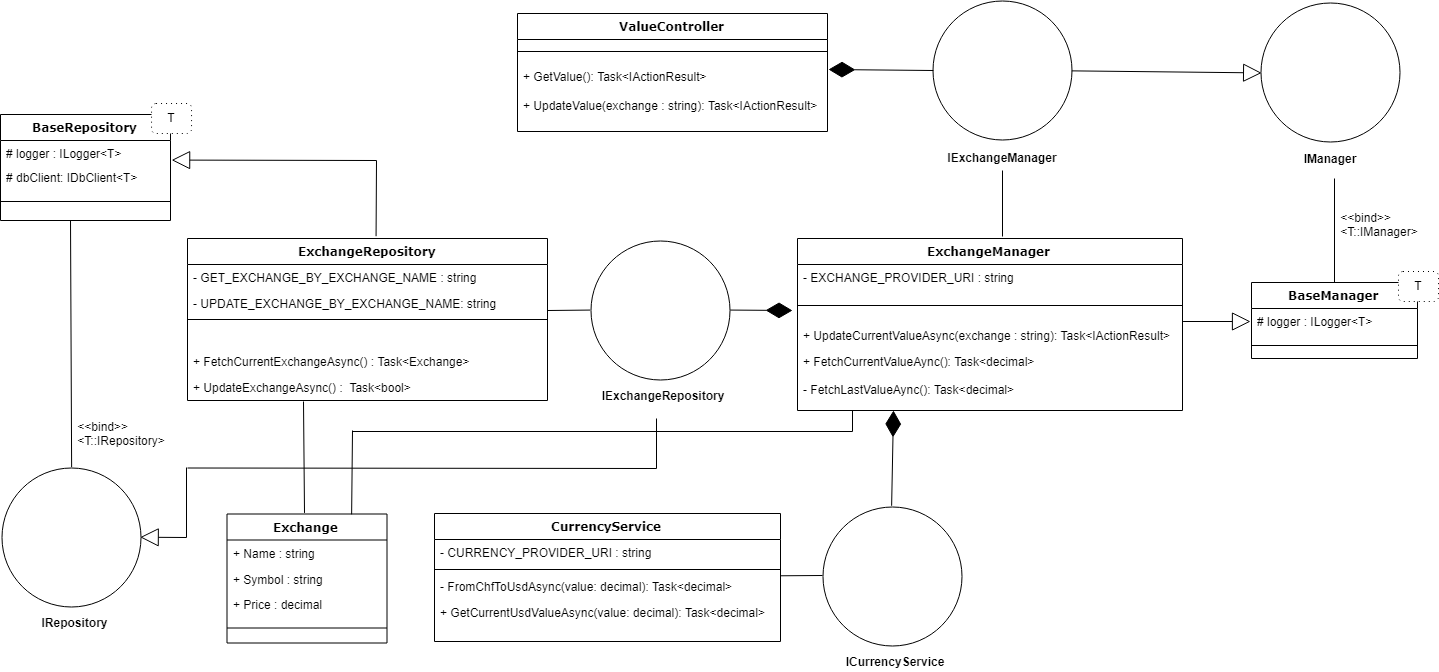
\includegraphics[width=\textwidth]{TkUMLClassDiagram.png}
        \caption{Diagramma delle classi del servizio Token Value}
    \label{fig:TkUMLClassDiagram}
\end{figure}

\subsubsection{Tecnologie}

Per il rispetto del requisito [\textbf{Vi001}] la scelta del linguaggio di programmazione da utilizzare è inevitabilemente ricaduta su \textit{C\#}.\\
Questo requisito è dovuto al fatto che l'intera piattaforma è stata sviluppata con la tecnologia \textit{.NET Framework} di \textit{Microsoft} e poggia sul \textit{Cloud Azure}, anch'esso sviluppato e mantenuto dalla stessa \textit{Microsoft}.\\
Questa scelta ha reso possible una perfetta integrazione del servizio con tutte le estensioni (\textit{Insight, Metrics etc.. }) e funzionalità aggiuntive messe a disposizione dalla piattaforma.\\\\
Lo stesso requisito ha inoltre imposto la creazione del database tramite l'utilizzo di \textit{PostgreSQL}. Questa è stata presa semplicemente per coerenza tecnologica con gli altri servizi che già utilizzavano la stessa tipologia di database.

\pagebreak
\subsection{Sviluppo}
Per comprendere a pieno l'andamento dello sviluppo del servizio è necessario innanzitutto dare una panoramica sia delle metodologie e dei \textit{tools} utilizzati dalla società che del \textit{Flow di sviluppo} imposto a tutti gli sviluppatori.

\subsubsection{Metodologia di sviluppo}
Data l'elevata preparazione tecnica e professionalità degli sviluppatori presenti nel \textit{team} di \textit{Sgame Pro} e vista la necessità di continui e rapidi miglioramenti dell'applicazione la società ha deciso di utilizzare una metodologia di sviluppo \textit{Agile} e, più in particolare, \textit{Scrum}.

\subsubsubsection{Scrum}
Il team di Sgame Pro utilizza il framework \textit{Scrum}, ossia un framework Agile, iterativo ed incrementale, per lo sviluppo di progetti complessi.\\
\textit{Scrum} si basa su tre pilastri fondamentali:
\begin{itemize}
	\item \textbf{Trasparenza}: I risultati dei precessi devono essere compresi dagli Stakeholders, ossia dagli individui direttamente responsabili del risultato del prodotto;
	\item \textbf{Verifica}: Le verifiche devono essere effettuate con bassa frequenza e da persone con competenze tecniche;
	\item \textbf{Adattamento}: Nel caso in cui il risultato di una o più verifiche identifichi un livello di qualità insoddisfacente, il processo di sviluppo deve essere modificato il prima possibile, al fine di riallineare il processo alle aspettative.
\end{itemize}
In \textit{Scrum} esiste ciò che viene formalmente definito lo \textit{Scrum Team}, il quale è formato da tre figure fondamentali:
\begin{itemize}
	\item \textbf{Product Owner}: responsabile della massimizzazione del valore del prodotto sviluppato dal \textit{Development Team};
	\item \textbf{Development Team}: formato dalle figure professionali che sviluppano effettivamente il prodotto;
	\item \textbf{Scrum Master}: coordina e supporta il \textit{Development Team}.
\end{itemize}
Durante il tirocinio il mio ruolo si posizionava all'interno del \textit{Development Team}, il quale veniva coordinato e supportato dallo \textit{Scrum Master} ed i quali \textit{output} venivano giudicati direttamente dal \textit{Product Owner}.\\
Il rispetto e l'attuazione di questo modello si riflette perfettamente nel processo di sviluppo aziendale, trattato dettagliamente nella sezione successiva.

\subsubsection{Processo di implementazione e rilascio}
La società \textit{Sgame SA} ha richiesto che il \textit{flow} di lavoro, durante l'implementazione di nuove \textit{features} di uno stesso servizio debba sempre utilizzare la seguente \textit{pipeline}:
\begin{enumerate}
	\item \textbf{Development};
	\item \textbf{UAT};
	\item \textbf{Staging};
	\item \textbf{Production}.
\end{enumerate}
La struttura sopra esposta segue fedelmente la struttura dei principali \textit{branch} riportata sull'apposito \textit{repository} presente in \textit{GitHub}.\\
Ad ogni punto sopra elencato corrispondono ambienti di sviluppo differenti, ognuno con uno scopo ben definito.\\\\
L'ambiente di \textit{Development} è dedicato esclusivamente all'implementazione di servizi, funzionalità e correzione degli errori (\textit{bug fix}).\\\\
\textit{UAT}, acronimo per \textit{User Acceptance Testing}, è utilizzato per il testing interno delle funzionalità e per l'approvazione interna del \textit{Product Manager}.\\\\
L'ambiente di \textit{Staging} è dedicato invece al \textit{Beta Testing}, ossia a test effettuati da personale esterno alla compagnia. Questo risulta estremamente efficace nello sviluppo di applicazioni mobile in quanto l'elevato numero di dispositivi presenti nel mercato richiede accertamenti (soprattutto lato \textit{UI}) sulla corretta visualizzazione e funazionamento delle nuove \textit{features}.\\\\
\textit{Production} è invece l'ambiente "esterno", ossia dove l'applicazione viene utilizzata dagli utenti di tutto il mondo.
%----------------------------------------------------------------------------------------
%	FIGURA 9
%----------------------------------------------------------------------------------------
\begin{figure}[h]
    \centering
    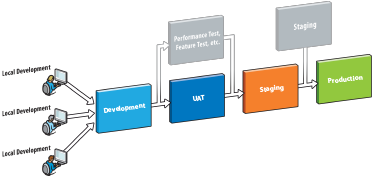
\includegraphics[scale=.85]{dev-flow.png}
        \caption{Processo di implementazione e rilascio in Sgame}
    \label{fig:dev-flow}
\end{figure}
\subsubsubsection{Processo di implementazione delle features}
Una volta iniziato il lavoro su una nuova \textit{feature} del servizio è necessario innanzitutto creare un nuovo \textit{branch} il cui nome deve tassativamente seguire la seguente struttura:\\\\
\textit{iniziali\_dello\_sviluppatore + nome\_feature}\\\\
%----------------------------------------------------------------------------------------
%	FIGURA 10
%----------------------------------------------------------------------------------------
\begin{wrapfigure}{r}{0.35\textwidth}
	\vspace{-50pt}
	\begin{center}
    	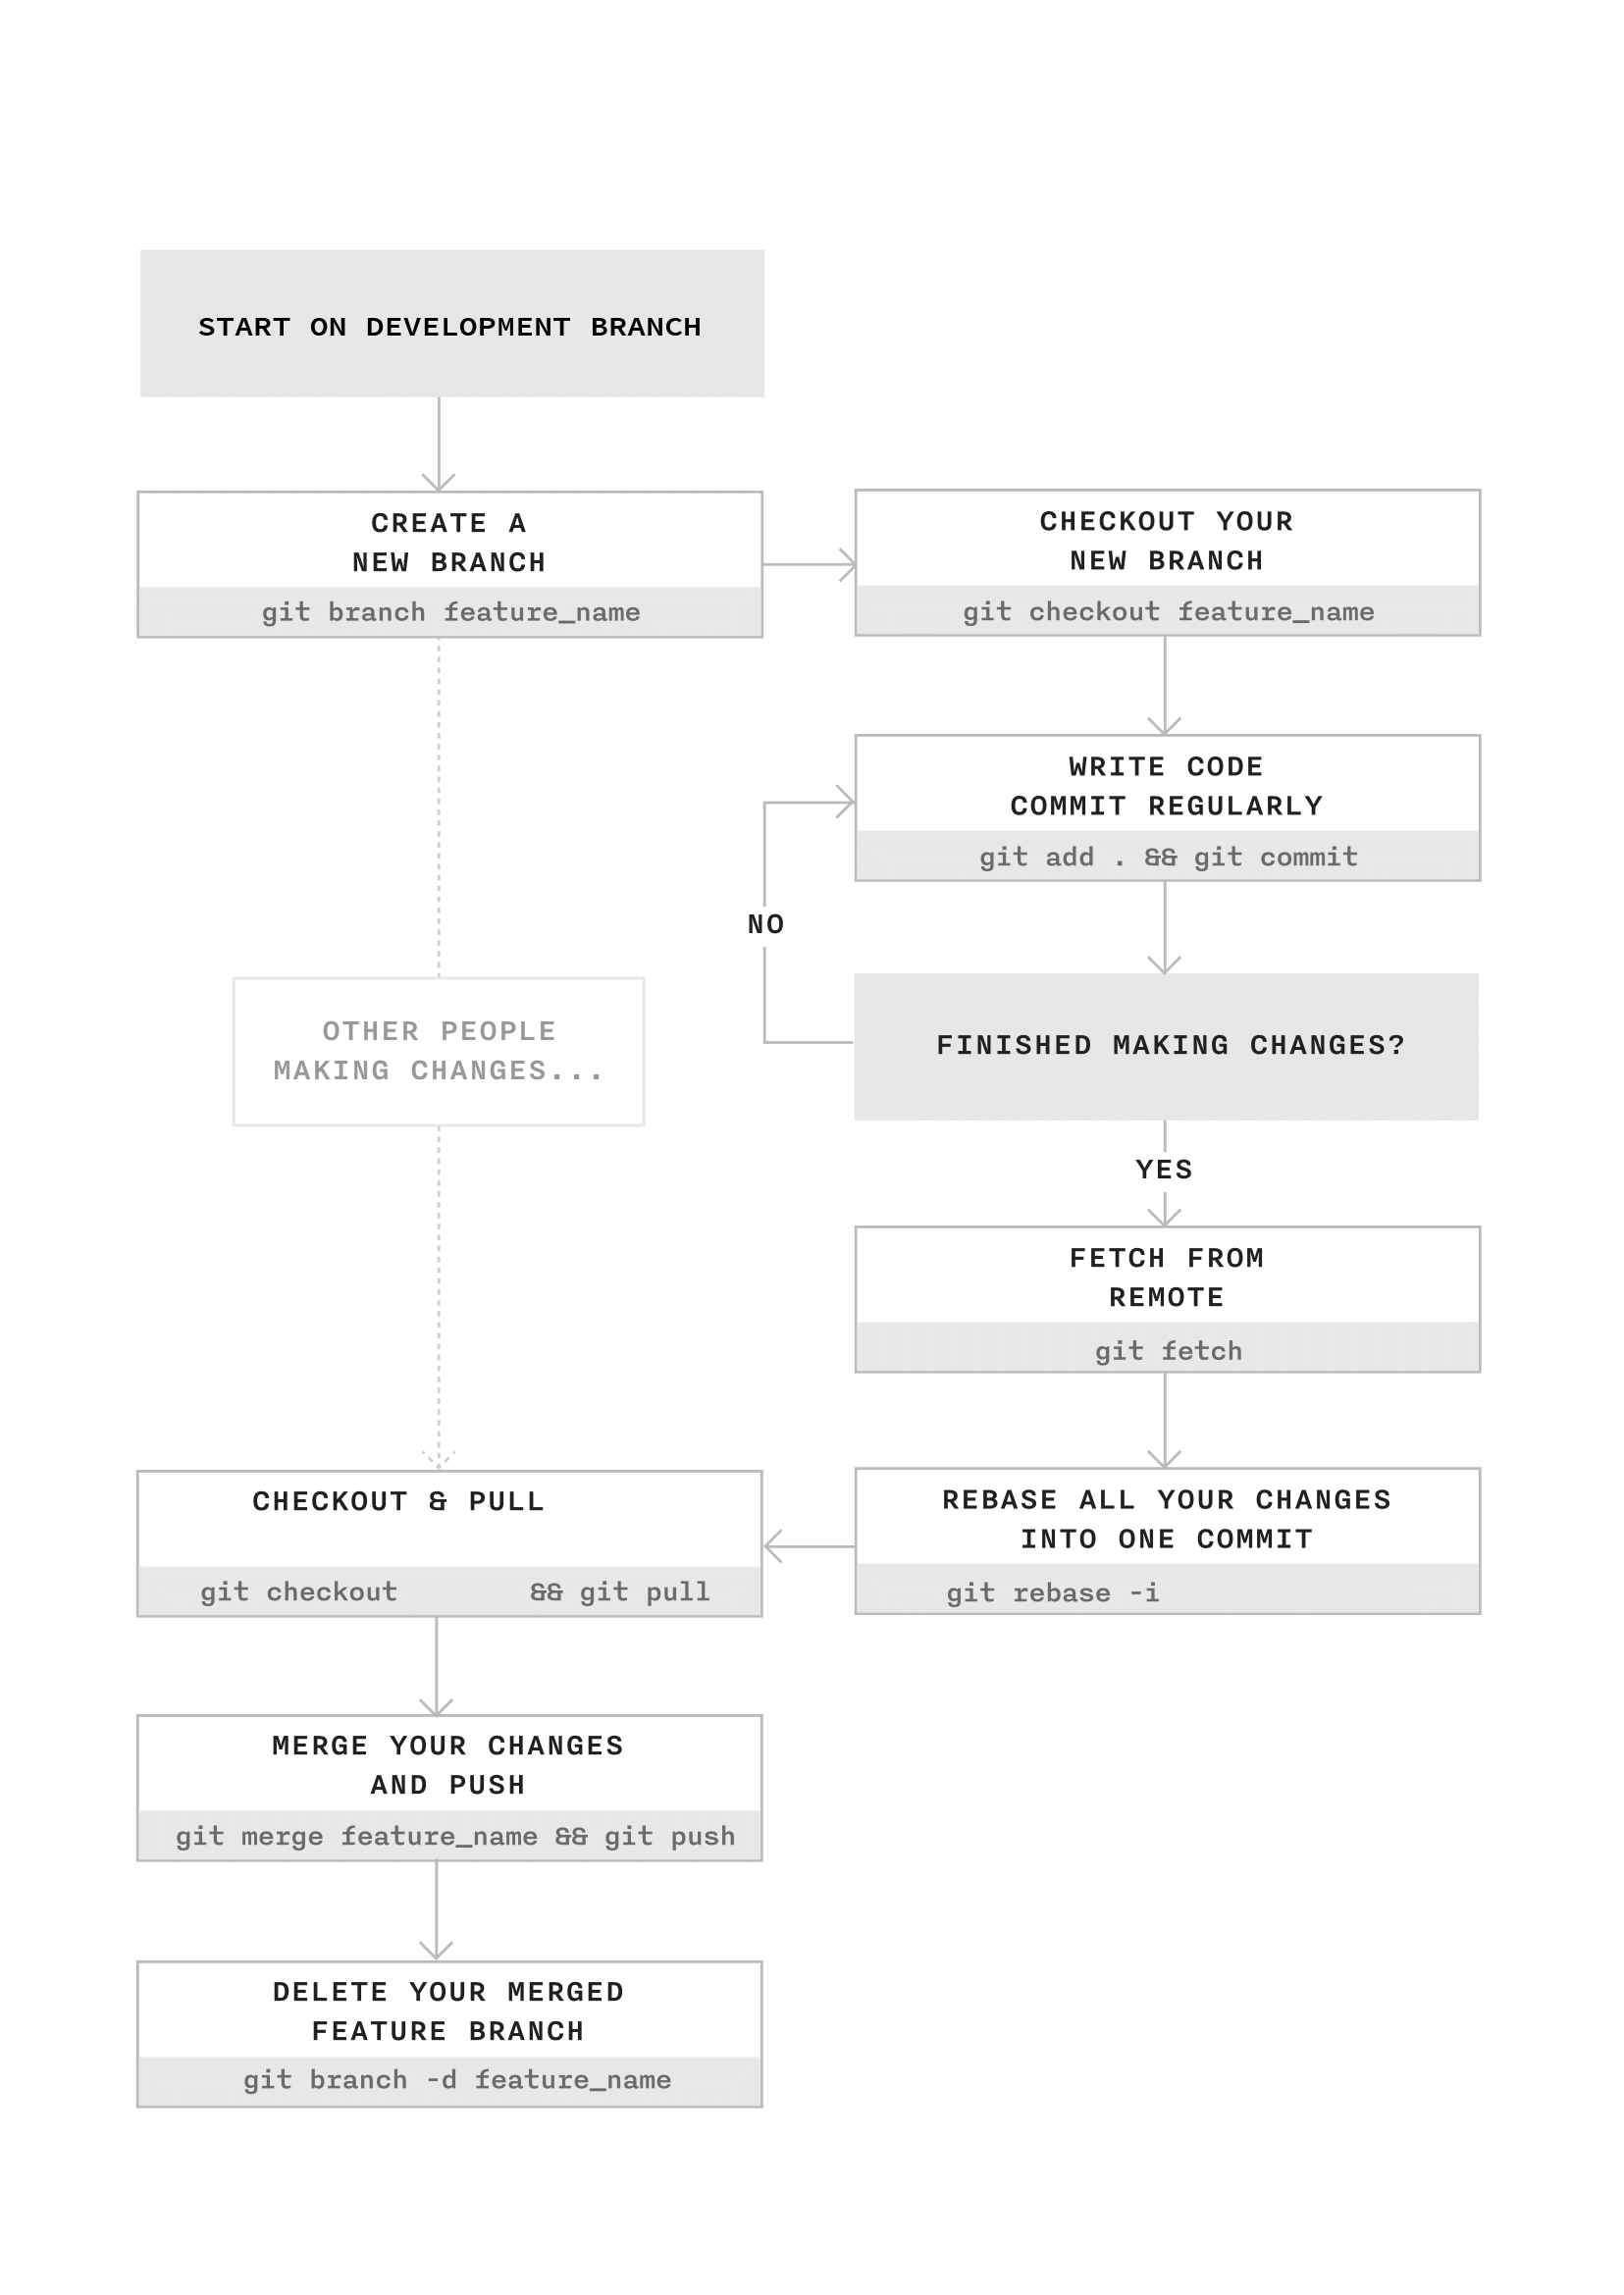
\includegraphics[width=0.4\textwidth]{git-flow.png}
  	\end{center}
  	\vspace{-10pt}
  	\caption{Implementazione di una feature}
  	\label{fig:git-flow}
  	\vspace{-9pt}
\end{wrapfigure}
Tutti i \textit{commit} riguardanti la stessa \textit{feature} andranno sempre ad utilizzare questo nuovo branch.\\
Una volta terminata, testata e validata la funzionalità o l'\textit{improvement} è necessario fare lo \textit{stash} di tutti i commit verso un unico commit che avrà (come \textit{commit message}) il nome della \textit{feature} stessa.\\
Questa andrà quindi inserita sul \textit{branch} di \textit{development} dopo aver effettuato il \textit{rebase}.\\\\
Il procedimento è invece differente quando, una volta implementata e testata una nuova funzionalità sull'ambiente di \textit{development}, questa vada inserita sull'ambiente di \textit{UAT}, \textit{Staging} e \textit{Production}.\\
L'unico modo per modificare il codice presente in uno di questi tre ambienti dedicati è tramite \textit{pull request}, il quale titolo deve essere tassativamente il nome della \textit{feature} che si va ad inserire.\\\\
Il rispetto di questo processo si rivela assolutamente necessario per permettere altri membri del team di effettuare \textit{Code review} sul codice che si intende inserire.\\
Questo permette un controllo efficace sul codice in ingresso nei vari ambienti tramite gli appositi sistemi di \textit{CI/CD}.

\pagebreak
\subsection{Integrazione}
Una volta completata l'implementazione del servizio \textit{Token Value} ed i relativi test funzinali e di unità, è stato necessario integrare il servizio con l'infrastruttura già esistente della piattaforma \textit{Sgame Pro}.\\\\
L'intero \textit{backend} dell'applicazione utilizza ciò che viene definito \textit{Cloud Computing}, ossia un sistema per la distribuzione di servizi di calcolo (\textit{server}), le risorse di archiviazione (\textit{database}) e reti, erogata tramite internet.
Il \textit{Cloud Computing} ha il vantaggio di offrire risorse estremamente flessibili ed un livello di scalabilità estremamente performante.\\\\
Il processo di integrazione è stato intrapreso dal \textit{DevOps} del team, seguendo le seguenti fasi:
\begin{itemize}
	\item creazione dell'istanza;
	\item configurazione dell'istanza;
	\item \textit{linking} con i \textit{repository} presenti su \textit{GitHub} per sfruttare la \textit{CI/CD}.
\end{itemize}
Dei tre passi sopra elencati solo l'ultimo ha riguardato da vicino il mio lavoro.\\
Infatti, tramite la \textit{CI/CD}, configurata con \textit{Microsoft Azure} e collegata direttamente ai \textit{repository} su \textit{GitHub}, il codice commitato veniva compilato, testato (tramite l'uso di test automatizzati) e pubblicato in forma completamente automatica.\\
Questo processo, oltre a velocizzare notevolmente lo sviluppo, ha permesso a me ed agli altri membri del team di testare il servizio fin da subito e di raccogliere fin da subito i \textit{feedback} dei \textit{Beta Testers}, oltre a quelli del \textit{Product Owner}.
%----------------------------------------------------------------------------------------
%	FIGURA 11
%----------------------------------------------------------------------------------------
\begin{figure}[h]
    \centering
    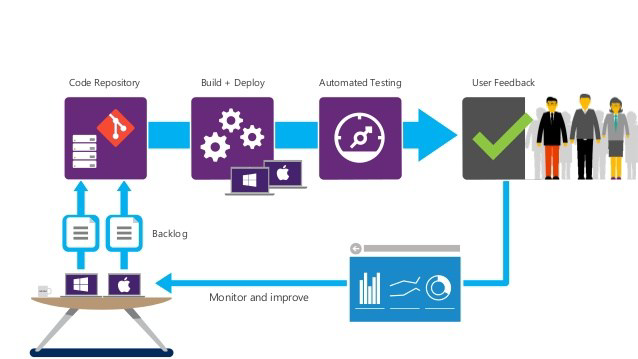
\includegraphics[scale=0.59]{ci-cd.png}
        \caption{Processo di CI/CD}
    \label{fig:ci-cd}
\end{figure}

\section{Ethereum Testnet}

\subsection{Overview}

Oltre allo sviluppo del servizio \textit{Token Value} al tirocinante è stato chiesto di testare integralmente le funzinalità dello \textit{Smart Contract} utilizzato dallo piattaforma.\\
Per farlo è stato necessario creare innanzitutto quella che viene definita una \textit{TestRPC}, ossia una rete locale che utilizza gli stessi protocolli della rete principale di \textit{Ethereum}, ma in cui le transazioni non richiedono l'esborso di denaro, ossia il pagamento di \textit{gas}.\\
In secondo luogo è stata invece configurata una \textit{Testnet Ropsten}, ossia una rete remota che, oltre ad utilizzare gli stessi protocolli della \textit{Mainnet} (\textit{Ethereum}), emula fedelmente le tempistiche ed i costi delle transazioni, ma la criptovaluta necessaria al pagamento delle \textit{gas fee} ha valore zero.\\
%----------------------------------------------------------------------------------------
%	FIGURA 12
%----------------------------------------------------------------------------------------
\begin{figure}[h]
    \centering
    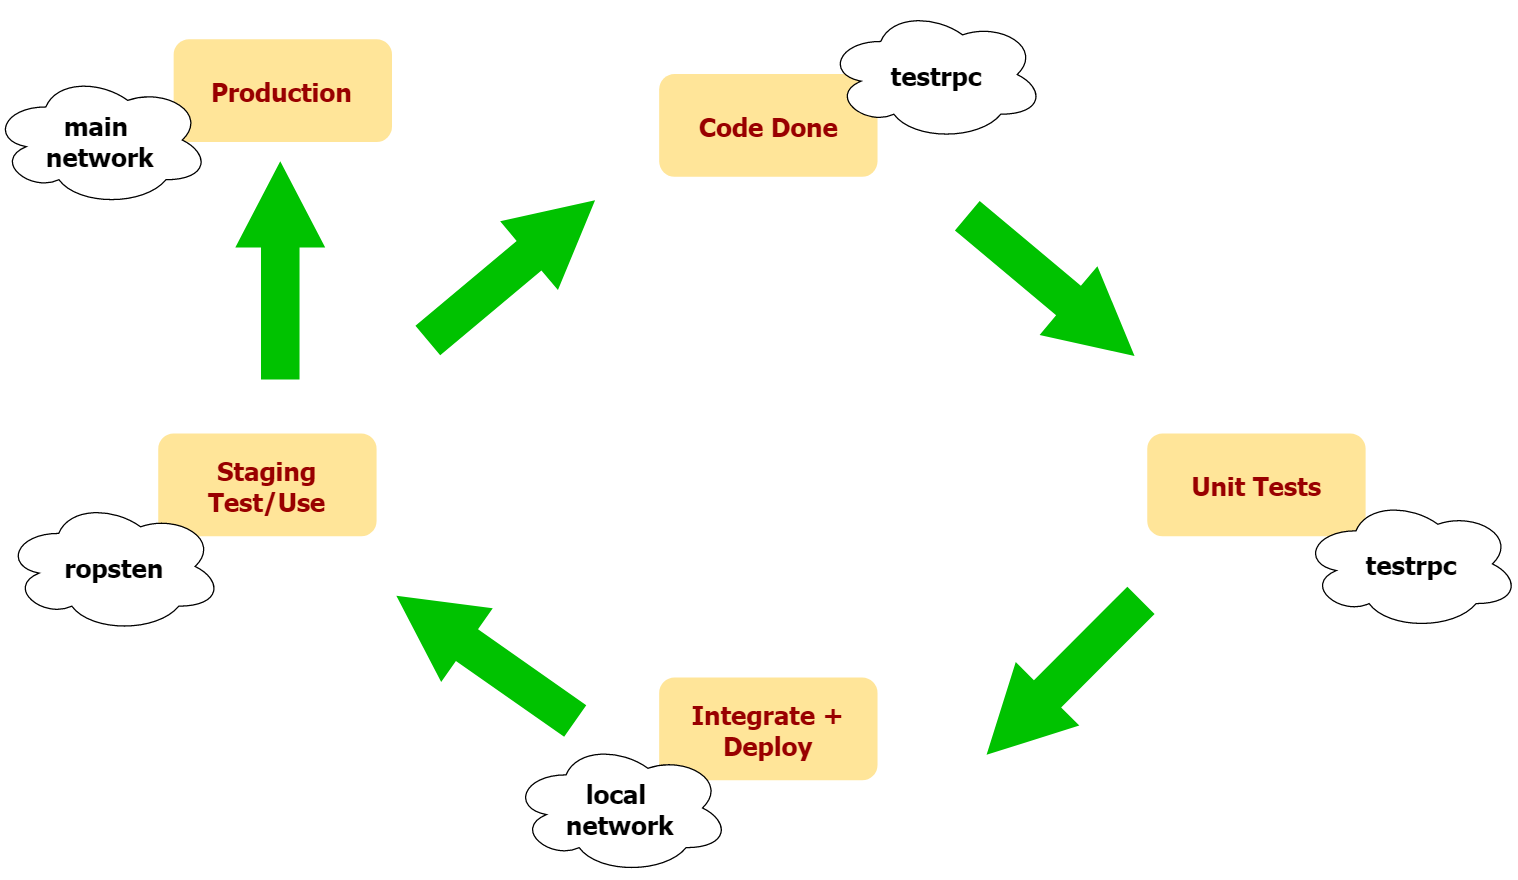
\includegraphics[scale=0.28]{testnet-diag.png}
        \caption{Processo di sviluppo, test e deploy in Ethereum}
    \label{fig:testnet-diag}
\end{figure}
\linebreak
Grazie all'ausilio di queste reti è quindi possibile testare lo \textit{Smart Contract}, verificandone ogni singola funzione per assicurarsi che il modello di business si rifletta sull'implementazione dello \textit{Smart Contract} stesso.
\pagebreak

\subsection{Pianificazione}

\begin{itemize}
	\item \textbf{Sesta Settimana}(42,5 ore) – Studio del servizio \textit{TX} e creazione dei diagrammi necessari a dimostrarne la comprensione;
	\item \textbf{Settima Settimana}(42,5 ore) – Creazione dell’ambiente di testing su \textit{Microsoft Azure} tramite l’utilizzo del tool \textit{Ganache} ed automazione del deploy dello \textit{Smart Contract} utilizzato dalla piattaforma Sgame; Utilizzo della rete pubblica \textit{Ropsten} per l'advanced testing dello \textit{Smart Contract} necessario al funzionamento della piattaforma \textit{Sgame Pro};
	\item \textbf{Ottava Settimana}(2,5 ore) – Presentazione agli \textit{Stakeholders} del lavoro svolto sul servizio \textit{Token Value}, comprensivo di documentazione e giustificazione delle soluzioni adottate dal tirocinante.\\
Presentazione agli Stakeholders del lavoro svolto sulle \textit{Testnet} ed esposizione dei risultati dei test.
\end{itemize}
\pagebreak
\subsection{Analisi dei requisiti}

Viene di seguito riportata la specifica dei requisiti richiesti per lo sviluppo e l'integrazione della rete di test per lo \textit{Smart Contract} sviluppato per la piattaforma \textit{Sgame Pro}.

\subsubsection{Specifica dei requisiti}

\textbf{Obbligatori}:
\begin{itemize}
	\item \textbf{Ob004} – l’ambiente testnet di tipo private deve utilizzare uno script di \textit{auto-deploy} per lo \textit{Smart Contract}.
\end{itemize}
\textbf{Vincolo}:
\begin{itemize}
	\item \textbf{Vi002} – l’ambiente \textit{testnet} di tipo \textit{private} deve utilizzare il tool \textit{Ganache}.
	\item \textbf{Vi003} – l’ambiente \textit{testnet} di tipo \textit{public} deve utilizzare il la rete \textit{Ropsten}.
\end{itemize}
\pagebreak
\subsection{TX Service}

\subsubsection{Overview}

Prima di poter configurare la \textit{Testnet} è stato necessario studiare il codice del servizio che la società ha chiamato \textit{TX}, necessario alla comunicazione con la rete \textit{Ethereum} e quindi con lo \textit{Smart Contract}.\\
Oltre alla comunicazione diretta con la \textit{blockchain} ed alla creazione ed invio delle transazioni su \textit{Ethereum}, \textit{TX} utilizza al suo interno un modulo di \textit{Anti-Fraud} basato sull'attribuzione dei punteggi ed un servizio ausiliario di \textit{Back Office} chiamato \textit{TX Admin}.\\
\textit{TX Admin}, grazie alla sua interfaccia grafica, permette il controllo e la verifica delle richieste di transazioni \textit{IN-OUT} da parte di un operatore.\\\\
Di seguito le funzionalità principali del servizio:
\begin{itemize}
	\item esecuzione delle transazioni verso indirizzi \textit{Ethereum} tramite l'utilizzo dello \textit{Smart Contract} creato per \textit{Sgame Pro};
	\item stime sui consumi di \textit{gas};
	\item verificare la validit' degli indirizzi di destinazione forniti;
	\item effettuare \textit{callback} al \textit{backend} della piattaforma per comunicare i cambiamenti di stato delle transazioni.
\end{itemize}
%----------------------------------------------------------------------------------------
%	FIGURA 14
%----------------------------------------------------------------------------------------
\begin{figure}[h]
    \centering
    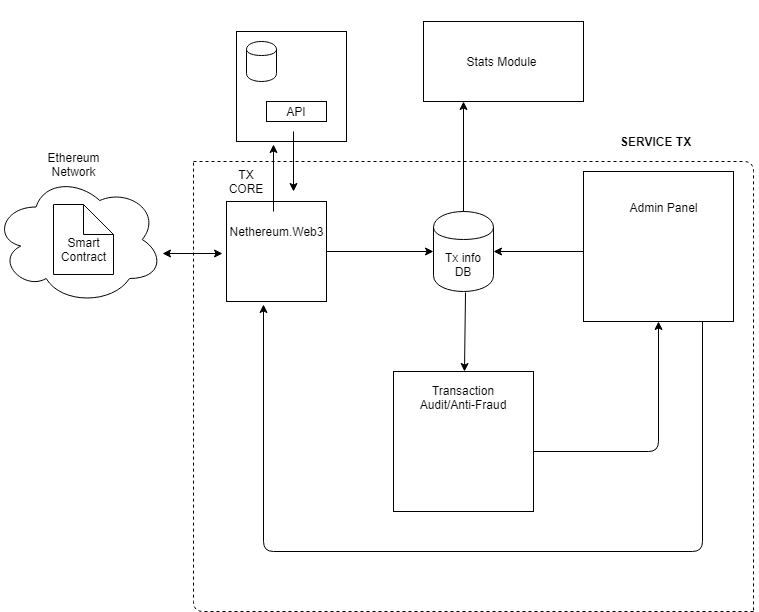
\includegraphics[scale=0.41]{tx-arch.png}
        \caption{Architettura semplificata del servizio TX}
    \label{fig:tx-arch}
\end{figure}
\pagebreak

\subsubsection{Specifiche}

La struttura di \textit{TX} ha rappresentato la traccia per quella che poi è diventata la struttura di \textit{Token Value}, e per questo ne condivide la separazione dei moduli in interfaccia e logica di business.\\
Anche in questo caso il servizio è composto da più moduli separati, ognuno con un compito specifico ed esplicitato in [\textbf{Figura~\ref{fig:tx-seq-diag}}].\\
%----------------------------------------------------------------------------------------
%	FIGURA 15
%----------------------------------------------------------------------------------------
\begin{figure}[h]
    \centering
    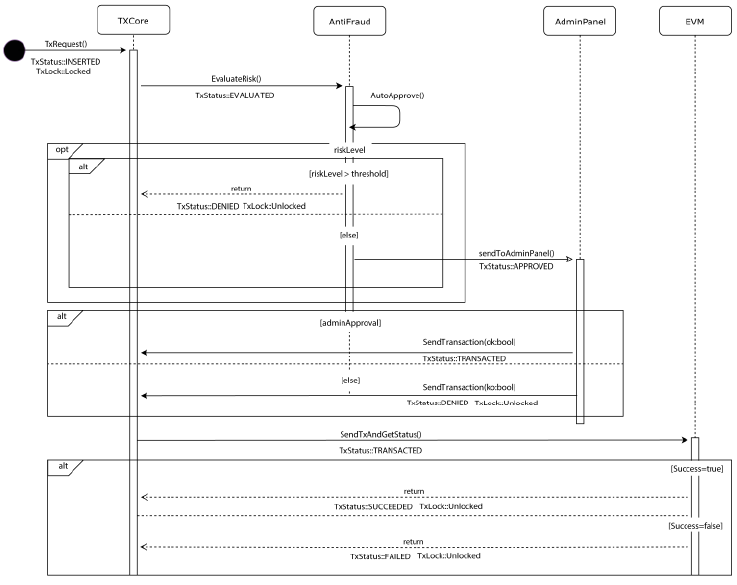
\includegraphics[scale=0.55]{tx-seq-diag.png}
        \caption{Diagramma di sequanza del servizio TX}
    \label{fig:tx-seq-diag}
\end{figure}
\linebreak
Ogni transazione passa quindi prima da un controllo \textit{Anti-Fraud}, per poi essere inviata al servizio \textit{TX Admin} o direttamente su \textit{Ethereum}.\\\\
Risulta quindi ora più chiaro come lo sviluppo della \textit{Tesnet Ethereum} è stato obbligatoriamente preceduto dallo studio della comunicazione tra il servizio \textit{TX} e la \textit{blockchain Ethereum}.

\pagebreak

\subsection{Private Tesnet}

Una \textit{private testnet}, come già spiegato in precedenza, è una rete locale che utilizza gli stessi protocolli della rete principale \textit{Ethereum}, ma in cui le transazioni vengono \textit{minate} (ossia validate ed inserite in un nuovo blocco) istantaneamente e non richiedono il pagamento di \textit{gas}.\\
Esistono più strumenti in grado di simulare una \textit{blockchain}, ma, per il rispetto del requisito di vincolo \textbf{Vi002}, la scelta è caduta inevitabilmente su \textit{testrpc}.\\\\
\textit{testrpc} è un client \textit{Ethereum}, basato su \textit{Node.js}, utilizzato per il test e lo sviluppo di \textit{dApps}. Esso utilizza \textit{ethereumjs}, una implementazione della \textit{EVM} in \textit{Javascript}, per simulare il comportamento della rete e rendere lo sviluppo di applicazioni basata su \textit{Ethereum} più semplice e veloce.

\subsubsection{Strumenti utilizzati}

\textit{Ganache} è l'ultima versione disponibile sul mercato di \textit{testrpc} e fa parte della \textit{Truffle Suite}, una collezione di strumenti (\textit{development environments, testing framework etc..}) estremamente utili per lo sviluppo di applicazioni decentralizzate.\\
%----------------------------------------------------------------------------------------
%	FIGURA 16
%----------------------------------------------------------------------------------------
\begin{figure}[h]
    \centering
    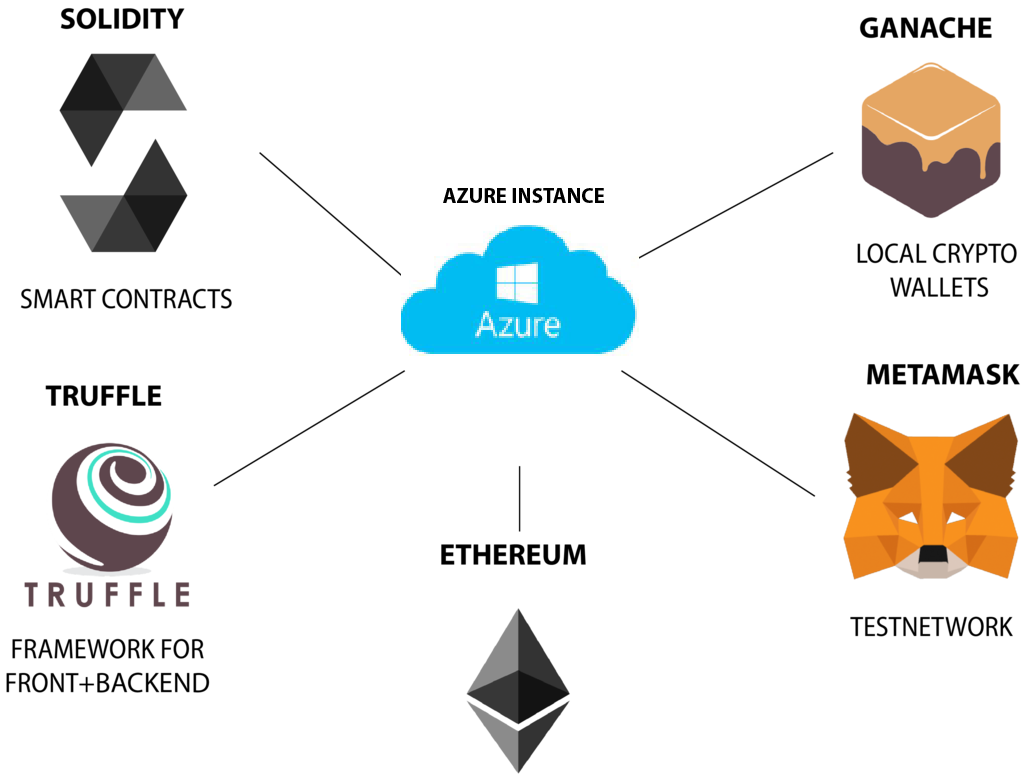
\includegraphics[scale=0.275]{eth-dev-test.png}
        \caption{Tools di sviluppo utilizzati dalle private networks}
    \label{fig:eth-dev-test}
\end{figure}
\linebreak
Il \textit{client} include tutte le funzioni \textit{RPC} più comuni (come gli eventi) e può essere eseguito in modo deterministico. Ciò previene il verificarsi di comportamente inattesi durante le transazioni e quindi un maggior controllo sulle stesse.\\\\

L'ultimo strumento necessario alla crezione della testnet prende il nome di \textit{METAMASK}, un "ponte" che permette di utilizzare direttamente dal proprio \textit{browser} un \textit{Ethereum full node} virtuale.

\subsubsection{Creazione}

La crezione di una \textit{testnet} di tipo \textit{private} è diventato un processo relativamente semplice negli ultimi due anni, grazie soprattutto all'elevato numero di \textit{tools} sviluppati (\textit{vedi sezione precedente}) ed al continuo miglioramento e semplificazione delle funzionalità associate.\\
Le difficoltà riscontrate sono quindi ricadute principalmente sulla comprensione del funzionamento ed delle interdipendenze che intercorrono tra i vari strumenti.\\\\
Poichè la rete di test si deve trovare necessariamente in locale ed i servizi atti alla comunicazione con la \textit{blockchain} si trovano in \textit{cloud} è stato necessario in prima battuta creare un'apposita istanza su \textit{Azure} dove "far girare" il server di \textit{testrpc}.\\
Una volta terminato il procedimento è stata necessaria l'installazione delle dipendenze ed infine l'installazione degli strumenti stessi.\\
%----------------------------------------------------------------------------------------
%	FIGURA 17
%----------------------------------------------------------------------------------------
\begin{figure}[h]
    \centering
    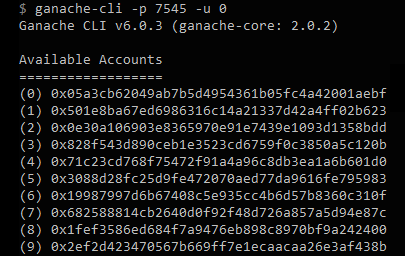
\includegraphics[scale=0.7]{ganache-cli.png}
        \caption{Creazione di una private network con Ganache-CLI}
    \label{fig:ganache-cli}
\end{figure}
\linebreak
A questo punto, dopo essersi collegati all'istanza tramite \textit{ssh} è semplicemente necessario avviare il server con il comando \textbf{\textit{ganache-cli}}, specificando la porta in ascolto (\textbf{\textit{-p 7545}}) e l'account che si desidera sbloccare (\textbf{\textit{-u 0}}).\\
In questo caso specifico il server starà in ascolto sulla porta \textit{7545} e si potrà utilizzare l'account \textit{0} (\textit{0x05a...ebf}) per poter interagire con lo smart contract.\\
Durante le fasi iniziali di test è stato necessario eseguire più \textit{deploy} \textit{Smart Contract} e, per evitare che i server esegua il \textit{reset} degli account a disposizione, è stata aggiunta l'opzione \textbf{\textit{-d}} (deterministic).

\subsubsection{Integrazione}

Per l'integrazione della testnet con il servizio \textit{TX} è stato necessario utilizzare una libreria \textit{wrapper}, chiamata \textit{Nethereum}, per scrivere il codice \textit{C\#} al fine di usare un'altra libreria (cosiderata uno \textit{standard} nella creazione di \textit{dApps}) che prende il nome di \textit{web3.js}.\\
\textit{web3.js} è, più propriamente, una collezione di librerie che consente di inviare \textit{Ether} da un account ad un altro, oltre a leggere e scrivere dati verso \textit{Smart Contract}.\\\\
Grazie all'utilizzo di questa libreria è stato necessario seguire quattro semplici passi:
\begin{itemize}
	\item prendersi nota dell'indirizzo (\textit{public key}) e della chiave privata (\textit{private key}) dell'account sbloccato con l'opzione \textbf{\textit{-u}} precedentemente passata al tool \textit{ganache-cli} e creare un apposito account.\\
	In questo modo si stà esplicitando l'indirizzo dell'account (in gergo \textit{owner}) autorizzato all'interazione con lo \textit{Smart Contract} e quindi alla firma delle transazioni tramite \textit{private key}.
	\begin{lstlisting}
// DEFINING ACCOUNT

    /* a private key is needed to sign the transactions.
     * The ethereum address is calculated from this private key 
     *  so each transaction signed with this key can be related to our ethereum addess
     */
    var privateKey = "dc925af9892df9f5f6f00dcbee5f6c59d53b631b32b475dfec49fabed8f57510";

    /* Who can do transactions, signing them with his private key */
    var senderAddress = "0x67af396FB49b054ad946a9E2cd67123750Fa1207";

    /* now it is possible to create an instance of Account which 
     * will be used to sign the transactions
     */
    var account = new Nethereum.Web3.Accounts.Account(privateKey);

    /* An instance of Web3 must be created to interact to the Ethereum client 
     * via RPC (remote procedure call).
     * [constructor public Web3(IAccount account, IClient client)] 
     * [client use ganache default port 8545] 
     */
    var web3 = new Web3(account, "HTTP://127.0.0.1:7545");
	\end{lstlisting}
	\item passare al servizio  \textit{Tx} i dati sopra elecanti, corredati dall'indirizzo dell'instanza creata e specificando la porta inserita come parametro sul tool \textit{ganache-cli} (\textbf{\textit{-p}}).
	\pagebreak
	\item utilizzare dell'indirizzo locale, il \textit{bytecode} e l'\textit{ABI} dello \textit{Smart Contract} appena \textit{deployato};
	\begin{lstlisting}
// DEFINING CONTRACT

    /* contract bytecode (for EVM) */
    var byteCode = "608...029";

    /* ABI (contract interface definition) */
    var abi = @"[{""constant"":true,""inputs"": ....... ,""type"":""event""}]";
	\end{lstlisting}
	\item effettuare il \textit{deploy} dello \textit{Smart Contract} di \textit{Sgame Pro};
	\begin{lstlisting}
// DEPLOYING CONTRACT

    /* creating _totalSupply to initialize SGM contract using BigInteger 
     * to pass the amount in wei (1 ETH = 10^18 wei)
     */
    System.Numerics.BigInteger totalSupply = System.Numerics.BigInteger.Parse("5000000000000000000");

    /* Now we deploy the smart contract using SGM's abi and bytecode.
     * The method send the initial transaction (SendRequest), 
     * aka call the SGM constructor, waits for the trasaction to be mined (AndAwait)
     * and finally returns the transaction receipt.
     * The transaction receipt of a newly deployed contract includes
     * the contract's address.
     * This address can be now used to interact with the contract itself. 
    */
    var receipt = await web3.Eth.DeployContract.SendRequestAndWaitForReceiptAsync(
        abi,                                              //contract's interface definition
        byteCode,                                         //contract's  bytecode
        senderAddress,                                    //deployer
        new Nethereum.Hex.HexTypes.HexBigInteger(900000), //gas
        null,
        totalSupply);                                     //SGM contructor parameter

	\end{lstlisting}
\end{itemize}
Alla fine della procedura il servizio \textit{TX} ha potuto comunicare con successo con lo \textit{Smart Contract} di \textit{Sgame pro}.\\
Questo ha permesso agli sviluppatori del serivizio di testare in prima persona tutte le funzionalità dello \textit{Smart Contract} e di creare una \textit{test suit ad-hoc} per accertarsi che la logica del serivizio rispettasse la logica di business.
\pagebreak

\subsection{Public Tesnet}

A differenza di una \textit{testnet} privata come \textit{testrpc}, una \textit{testnet} pubblica ha la peculiarità di essere in tutto e per tutto una \textit{blockchain}, con l'unica differenza che la criptovaluta utilizzata al suo interno non ha nessun valore.\\
%----------------------------------------------------------------------------------------
%	FIGURA 18
%----------------------------------------------------------------------------------------
\begin{wrapfigure}{r}{0.35\textwidth}
	\vspace{-31pt}
	\begin{center}
    	
\includegraphics[width=0.1\textwidth]{ropsten-logo.png}
  	\end{center}
  	\vspace{-10pt}
  	\caption{Ropsten Logo}
  	\label{fig:ropsten-logo}
\end{wrapfigure}
Per il rispetto del requisito \textbf{Vi003} la scelta è ricaduta obbligatoriamente sulla rete \textit{Ethereum Ropsten}.\\
\textit{Ropsten}, come le altre \textit{testnet} pubbliche, è utilizzata dagli sviluppatori di \textit{Ethereum} di tutto il mondo per testare gli \textit{Smart Contract} e tutti i servizi di interazione con la \textit{blockchain Ethereum}.\\
Per poterla utilizzare è innanzitutto necessario procurarsi degli \textit{rETH}, che altro non sono che la criptovaluta utilizzata per il pagamento delle transazioni all'interno della rete \textit{Ropsten} stessa.\\
Ricevere \textit{rETH} è un procedimento estremamente semplice.
Basta infatti utilizzare quelli che vengono definiti \textit{faucet} (rubinetti), ossia delle pagine web dove, una volta inserito l'indirizzo del proprio \textit{wallet Ropsten}, è possibile ricevere gratuitamente uno o più \textit{rETH}.\\\\
Testare in una rete pubblica è estremamente differente che testare in una rete privata, anche se il risultato è lo stesso.\\
Essendo una rete pubblica un agglomerato di nodi sparsi in tutto il mondo e connessi via internet, per accedervi sono applicabili due strade:
\begin{itemize}
	\item diventare un \textit{full node}, ossia scaricare lo storico di tutte le transazioni avvenute nella rete \textit{Ropsten}, partendo dal \textit{Genesis Block} (~80Gb);
	\item utilizzare un client che attui da interfaccia alla \textit{blockchain} e che emuli un \textit{full node}.
\end{itemize}
Ovviamente scelta è ricaduta sulla seconda opzione ed il tool utilizzato è stato \textit{METAMASK}.\\
L'enorme comodità di \textit{METAMASK} è che può essere utilizzato direttamente da \textit{browser} (esiste un famoso \textit{add on} per \textit{Google Chrome}) ed è estremamente facile da utilizzare.
\pagebreak

\subsubsection{Integrazione}
Prima di poter utilizzare la rete \textit{Ropsten} con il serivizio \textit{TX} è stato necessario effettuare un nuovo \textit{Deploy} dello \textit{Smart Contract} sulla rete stessa.\\
Il procedimento è abbastanza semplice una volta capite le logiche di rialscio, ma è richiesta comunque molta attenzione durante la procedura poichè, una volta pubblicato sulla rete, lo \textit{Smart Contract} diventa pubblico e non è più possible rimuoverlo (ovviamente).\\
%----------------------------------------------------------------------------------------
%	FIGURA 19
%----------------------------------------------------------------------------------------
\begin{figure}[h]
    \centering
    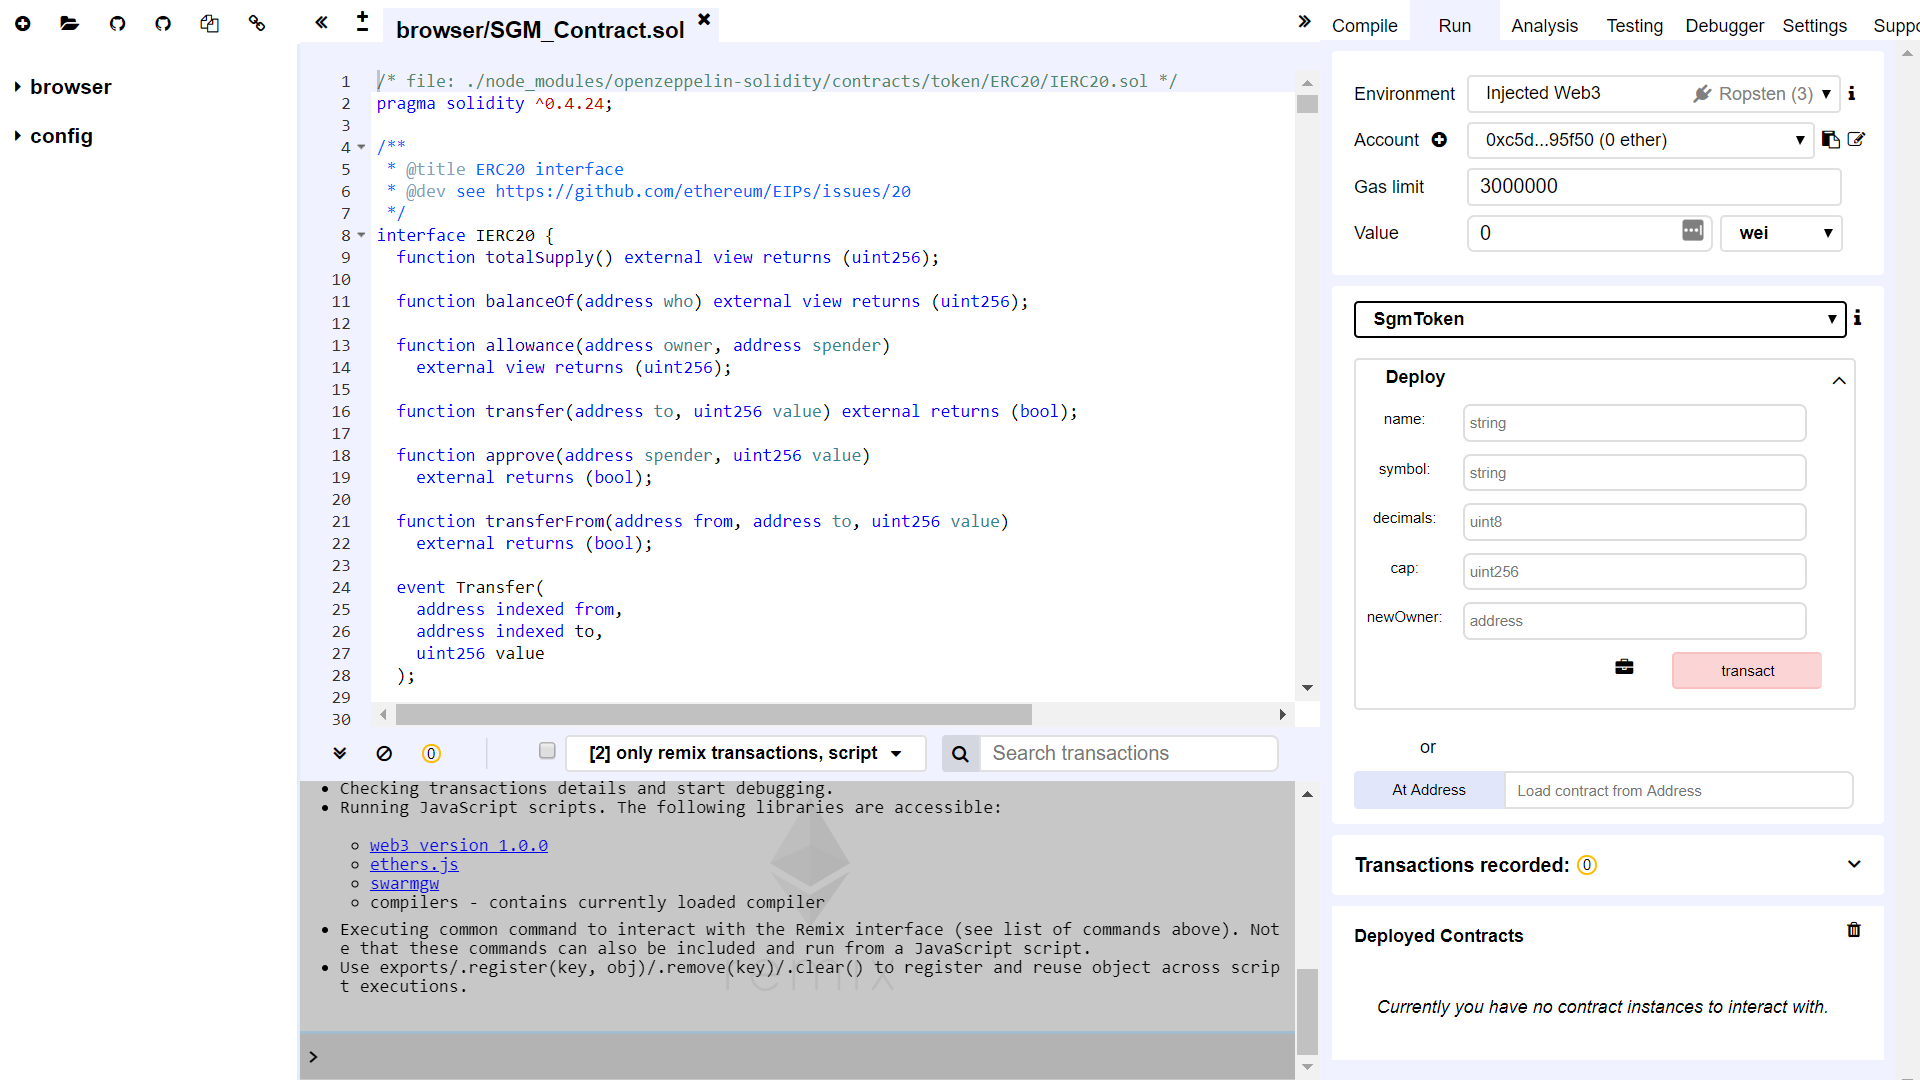
\includegraphics[scale=0.4]{sgm-contract-deploy.png}
        \caption{Deploy dell'SGM Contract tramite Remix-IDE}
    \label{fig:sgm-contract-deploy}
\end{figure}
\linebreak
Esistono più metodi per farlo ma, quello sicuramente più veloce ed intuitivo, è tramite il tool \textit{Remix IDE}.\\
\textit{Remix IDE} è un \textit{IDE} online ed usufruibile direttamente da \textit{browser} per la creazione, pubblicazione ed interazione con gli \textit{Smart Contract}.\\
Al suo interno è possibile utilizzare direttamente \textit{METAMASK} e ciò si traduce in un'incredibile risparmio di tempo.\\
Una volta terminato il \textit{deploy} è stato necessario inserire nel servizio \textit{TX} le medesime informazioni (aggiornate) utilizzate per \textit{testrpc}, con l'unica differenza che l'indirizzo con il quale viene istanziato \textit{web3} necessita di un servizio ponte chiamato \textit{Infura}.\\
\textit{Infura} funziona esattamente come \textit{METAMASK} ma, a differenza di quest'ultimo, può essere integrato direttamente in un servizio grazie alle numero \textit{API} che mette a disposizione.\\\\
Una volta terminato il procedimento è stato possibie testare lo \textit{Smart Contract} di  \textit{Sgame Pro} direttamente dal servizio \textit{TX} e di conseguenza testare le prime transazioni direttamente dall'aaplicazione mobile.

\section{Considerazioni finali}

In questo capitolo verrà svolta un’analisi a posteriori dell’attività di tirocinio svolta in \textit{Sgame pro}.\\
Verranno di seguito elencati conoscenze acquisite ed obiettivi raggiunti durante lo svolgimento dei progetti di \textit{stage}.

\subsection{Conoscenze acquisite}

Tenendo conto del tempo avuto a disposizione, il quantitativo di conoscenze acquisite durante il tirocinio in \textit{Sgame SA} è stato davvero enorme.\\
Il risultato ottenuto non è stato però solo il frutto di insegnamenti diretti da parte del team di sviluppo di \textit{Sgame Pro}, ma soprattutto di un ingente sforzo personale nello studio diretto dello \textit{stack} di tecnologie utilizzate dall'azienda.\\
La scelta del progetto di \textit{stage} è stata enormemente influenzata dalla possibilità di toccare con mano l'utilizzo della \textit{blockchain}, tecnologia per me di assoluto interesse fin dagli inizi del terzo anno accademico (Ottobre 2017).\\
Ho appreso e consolidato lo sviluppo di applicazioni decentralizzate utilizzanti \textit{Ethereum}, oltre che ad approfondire l'affascinante mondo delle \textit{public blockchain}, delle \textit{ICO} e delle relazioni che intercorrono tra lo sviluppo di un prodotto software e gli obiettivi di business ad esso associati.\\\\
\`E inoltre doveroso citare la `scoperta` del \textit{framework .NET} e del linguaggio \textit{C\#}, il quale non è mai stato preso in considerazione nei miei studi ed interessi extra scolastici.
A mio avviso \textit{Microsoft} stà diventando sempre più un riferimento nello sviluppo software, grazie principalmente ai numerosi ed innovativi servizi offerti da \textit{Azure} ed ai continui aggiornamenti del \textit{framework .NET}.

\subsection{Obiettivi raggiunti}

La crezione di un servizio totalmente realizzato da me è stata inizialmente una sfida, diventando poi un bellissimo traguardo personale.\\
L'enorme differenza tra il lavoro in azienda e lo sviluppo software a fini didattici ha fatto sì che il mio impegno nella progettazione e nello sviluppo del servizio (sempre guidato dal team di sviluppo interno) raggiungesse livelli impensabili, al fine di non deludere le aspettative che la società ha riposto in me con l'assegnazione di un elemento così centrale nel successo della piattaforma stessa.\\\\
La creazione e l'integrazione delle \textit{testnet} ha fatto sì che entrassi in contatto diretto con una tecnologia che a mio avviso sarà sempre più utilizzata fino a che diverrà indispensabile nella vita di tutti i giorni.\\
Posso ad oggi affermare di far parte di un ristretto gruppo di svilupattori che ha avuto l'opportunità di lavorare direttamente su \textit{Ethereum} a livello business e questo, tra le altre cose, mi rende estremamente orgoglioso del lavoro svolto in \textit{Sgame SA} durante il mio tirocinio. 

\pagebreak
\bibliographystyle{abbrv}
\bibliography{thesis}

\end{document}
